
% \documentclass[final,5p,times]{elsarticle}
\documentclass[final,5p,times,twocolumn]{elsarticle}


\usepackage{graphicx}%
\usepackage{multirow}%
\usepackage{amsmath,amssymb,amsfonts}%
\usepackage{amsthm}%
\usepackage{mathrsfs}%
\usepackage[title]{appendix}%
\usepackage{xcolor}%
\usepackage{textcomp}%
\usepackage{manyfoot}%
\usepackage{booktabs}%
\usepackage{algorithm}%
\usepackage{algorithmicx}%
\usepackage{algpseudocode}%
\usepackage{listings}%
\usepackage{threeparttable}%
\usepackage{caption}
\usepackage{url}
\usepackage{tabularx}

\captionsetup{font=normalsize}

%% The amsthm package provides extended theorem environments
% \usepackage{amsthm}

%% The lineno packages adds line numbers. Start line numbering with
%% \begin{linenumbers}, end it with \end{linenumbers}. Or switch it on
%% for the whole article with \linenumbers.
%% \usepackage{lineno}

\journal{Journal of \LaTeX\ Templates}

\begin{document}

\begin{frontmatter}

    \title{Efficient Implementations of CRAFT Cipher For Internet of Things }

    \author[]{Jiahao Xiang}
    \author[]{Lang Li\corref{cor1}}
    % \author[a,b]{Jiahao Xiang}
    % \author[a,b]{Lang Li\corref{cor1}}

    \ead{lilang911@126.com}

    \cortext[cor1]{Corresponding author}

    % \affiliation[a]{organization={College of Computer Science and Technology},%Department and Organization
    %     addressline={Hengyang Normal University},
    %     city={Hengyang},
    %     postcode={421002},
    %     state={},
    %     country={China}}

    % \affiliation[b]{organization={Hunan Provincial Key Laboratory of Intelligent Information Processing and Application},%Department and Organization
    %     addressline={Hengyang Normal University},
    %     city={Hengyang},
    %     postcode={421002},
    %     state={},
    %     country={China}}



    \begin{abstract}
        The rapid growth of the Internet of Things (IoT) highlights the importance of lightweight cryptography in maintaining security.
        However, enhancing performance while ensuring the same level of security remains a significant challenge.
        This paper presents two innovative architectures for the CRAFT lightweight block cipher, aiming to enhance performance without compromising security.
        The novel Serial and Unrolled architectures are introduced to achieve low area usage and high throughput, respectively.
        Specifically, the Serial architecture reduces the datapath from 64-bit to 4-bit, significantly decreasing the area.
        The Unrolled architecture, on the other hand, minimizes latency from 32 to 16.
        Additionally, Boolean satisfiability (SAT) solvers are employed to identify a lower-cost area implementation of the S-Box.
        The proposed designs underwent evaluation on three distinct FPGA platforms: Artix-7, Kintex-7, and Spartan-7.
        The results suggest that the low area design reduces area usage by 15.82\% compared to the PRESENT cipher.
        On the other hand, the unrolled design doubles the throughput rate at 100MHz and significantly reduces energy consumption per bit by 47.89\% compared to the PRESENT cipher.
        To the best of our knowledge, the low area design sets a new area record on the FPGA configured with a 64-bit block size and 128-bit key size.
        Therefore, the proposed designs could offer enhanced performance while maintaining security for IoT devices.
    \end{abstract}


    \begin{keyword}
        %% keywords here, in the form: keyword \sep keyword
        Internet of Things  \sep Lightweight block cipher \sep Field-programmable gate array(FPGA)\sep  Low-area, High-throughput
        %% PACS codes here, in the form: \PACS code \sep code

        %% MSC codes here, in the form: \MSC code \sep code
        %% or \MSC[2008] code \sep code (2000 is the default)
    \end{keyword}

\end{frontmatter}

%% \linenumbers

%% main text


\section{Introduction}\label{sec1}

The Internet of Things (IoT) is rapidly integrating into various aspects of everyday life.
With this advancement, a growing number of security issues are emerging.
These security concerns are extensively discussed in \cite{Meneghello2019a}.
To ensure data protection, the cryptography techniques outlined in \cite{Swessi2022} are recommended.

However, the resource constraints of many IoT devices pose challenges for the implementation of robust security measures. These devices often have limited memory, processing power, and energy. Therefore, the security measures need to be lightweight to ensure they do not overburden the resources. Lightweight cryptography, a subset of cryptography, provides solutions specifically designed for these resource-limited devices, as discussed in \cite{Mohajerani2020}.

The field of lightweight cryptography has received considerable attention in recent years. Examples of this include PRESENT \cite{Bogdanov2007}, LED \cite{Guo2011}, Midori \cite{Banik2015a}, QTL \cite{Li2016}, GIFT \cite{Banik2017}, CRAFT \cite{Beierle2019}, Shadow \cite{Guo2021}, DULBC \cite{Yang2022}, IVLBC \cite{Huang2023}, BipBip \cite{Belkheyar2023}, and LELBC \cite{Song2024}. More ciphers can be found in \cite{Zakaria2023}. The implementation of lightweight ciphers for various applications has also been widely studied.

Efficient implementation allows lightweight ciphers to be used in various settings.
A hardware implementation can enhance the performance of these ciphers in resource-limited environments.
Several researchers have proposed different architectures and optimizations for various ciphers.
Lara-Nino et al. \cite{LaraNino2017} introduced a 16-bit datapath architecture for the PRESENT cipher, reducing both the area and power consumption.
Pandey et al. \cite{Pandey2019} suggested an optimized key schedule of PRESENT, which resulted in a smaller area.
Shahbazi et al. \cite{Shahbazi2021} proposed an 8-bit serial architecture for AES, also reducing the area and power consumption.
Li et al. \cite{Li2021} presented unrolled architectures and a low-cost architecture for PRINCE, separately optimizing the throughput and area.
Bharathi et al. \cite{Bharathi2022} enhanced the performance of the PRESENT cipher by expanding the key length.
Lastly, Yang et al. \cite{Yang2023} shared components in the cipher process for LILLIPUT, resulting in a smaller area.


This work presents the first implementation of CRAFT on FPGA platforms.
Two architectures for CRAFT, Serial and Unrolled, are proposed. The Serial architecture reduces the datapath from 64-bit to 4-bit, meaning it only uses one S-Box, which significantly reduces the area usage.
The Unrolled architecture reduces the latency of the encryption process, thereby improving the throughput rate.
The optimal implementation of the S-Box, aimed at further area reduction, is determined using a SAT solver in conjunction with the GEC encoding scheme.
The experiments are conducted on three different FPGA platforms: Artix-7, Kintex-7, and Spartan-7.
The source code for the proposed designs is available online.\footnote{\url{https://github.com/xjh2000/craft_implementation}}
The main contributions of this article are as follows.
\begin{itemize}
    \item Two architectures for CRAFT, Serial and Unrolled, are proposed. These are optimized for area and throughput, respectively.
          The Serial architecture reduces the area usage by 15.72\% compared to the work of Bharathi et al. \cite{Bharathi2022}.
          The Unrolled architecture doubles the throughput rate compared to the same work.
    \item The optimal implementation of the S-Box, which results in further area reduction, is identified using a SAT solver.
          The proposed S-Box implementation achieves a 28.9\% area reduction compared to the work of Bao et al. \cite{bao2019peigen}.
    \item The architectures are implemented across three different FPGA platforms: Artix-7, Kintex-7, and Spartan-7. This variety allows engineers to select the platform that best suits their application needs.
\end{itemize}


The remainder of this article unfolds as follows: Section~\ref{sec2} delves into the specifics of CRAFT. The duo of proposed architectures for CRAFT are explored in Section~\ref{sec3}. Section~\ref{sec4} lays out the metrics and environment used for experimental evaluation. An in-depth performance analysis of all the architectures is presented in Section~\ref{sec5}. Lastly, Section~\ref{sec6} encapsulates the work done and points towards potential avenues for future research.

\section{Specification of CRAFT}\label{sec2}

CRAFT is a lightweight tweakable block cipher that operates on a 64-bit plaintext size, a 128-bit key size, and a 64-bit tweak size.
It outputs a 64-bit ciphertext.
The confusion and diffusion properties of CRAFT ensure that the distribution of probabilities between the plaintext and ciphertext is independent.
For more details on CRAFT, refer to Figure~\ref{fig1} which depicts its architecture.
The encryption process of CRAFT is outlined in Algorithm~\ref{alg1}.
The decryption process is similar to the encryption process, with the only difference being that the round keys are applied in reverse order.
The main notations used throughout this paper are outlined in Table~\ref{tab1}.


\begin{table}[h]
    \centering
    \caption{Main Notations}\label{tab1}%
    \begin{tabular}{|c|l|}
        \hline
        Notation & Description                           \\
        \hline
        $TK_i$   & tweakeys used in the $i^{th}$ round   \\
        $RC_i$   & round constant for the $i^{th}$ round \\
        $R_i$    & Function for the $i^{th}$ round       \\
        $SB$     & Sub-Box                               \\
        $MC$     & Mix-Columns                           \\
        $PN$     & PermuteNibbles                        \\
        $PK$     & Permutation used in key schedule      \\
        $\oplus$ & XOR operation                         \\
        $||$     & Concatenation operation               \\
        $\sim$   & Inverse operation                     \\
        $\land$  & And operation                         \\
        $\lor$   & Or operation                          \\
        \hline
    \end{tabular}
\end{table}

\begin{figure}[h]%
    \centering
    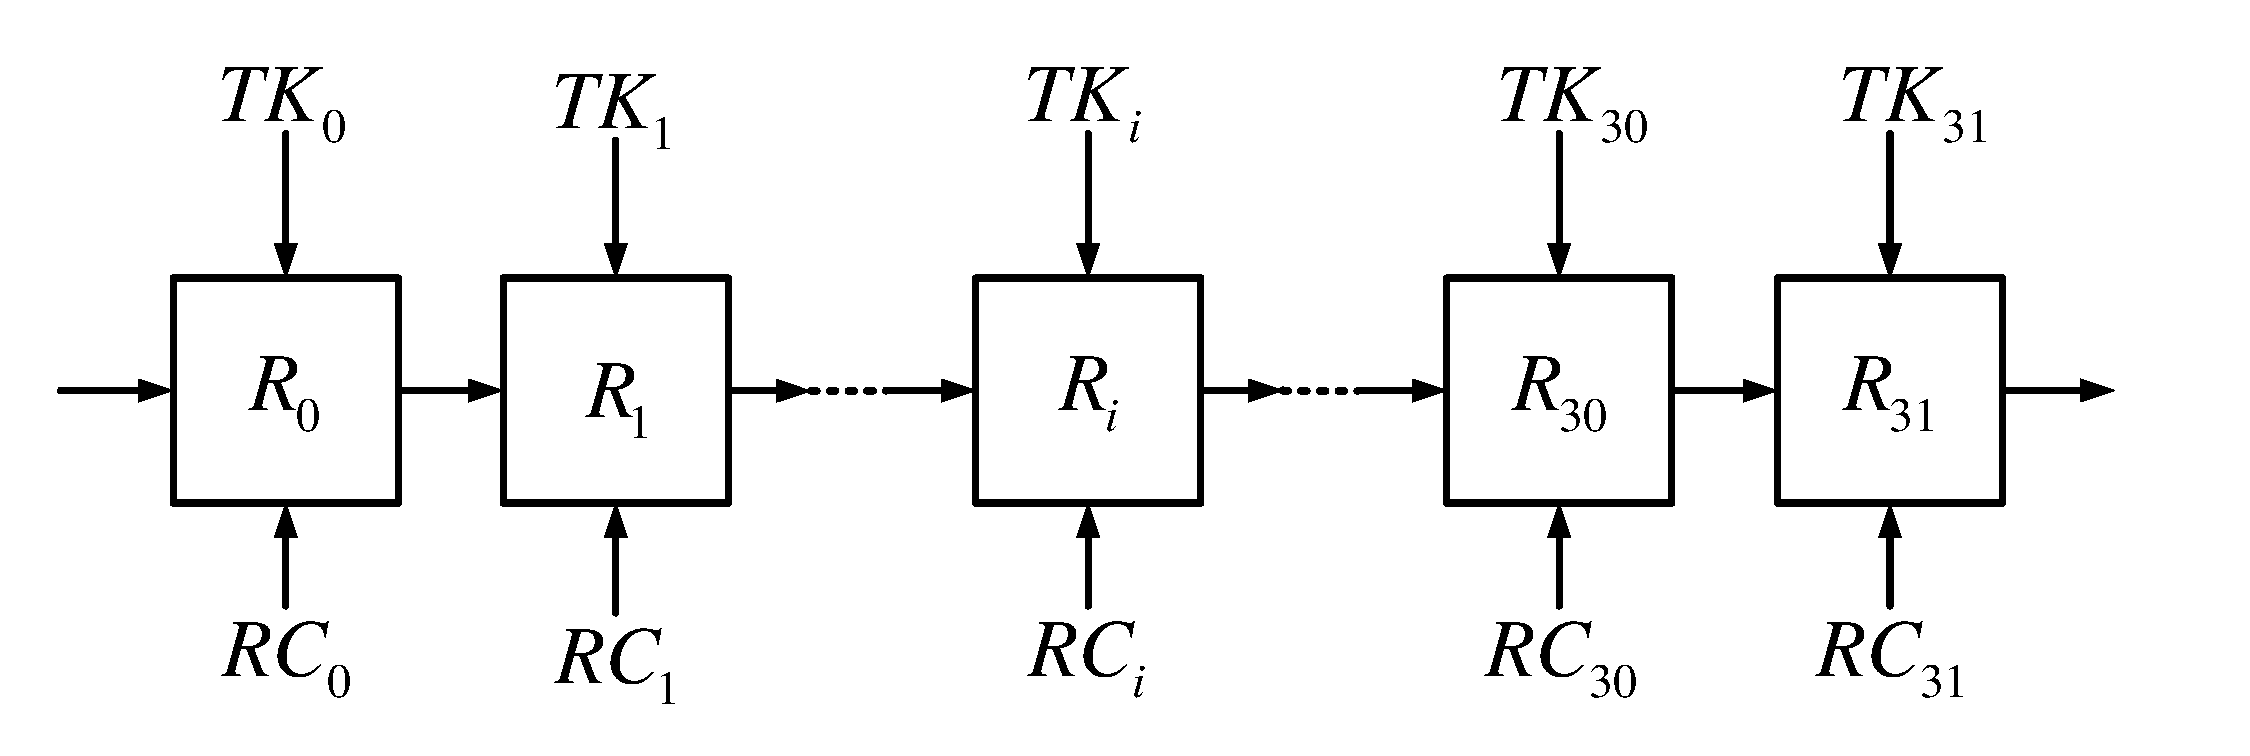
\includegraphics[width=0.45\textwidth]{./fig/struct-craft.pdf}
    \caption{Architecture of CRAFT}\label{fig1}
\end{figure}

\begin{algorithm}[h]
    \caption{CRAFT Encryption Process}\label{alg1}
    \textbf{Input:} Plaintext $P$, Key $K_0||K_1$, Tweak $T$ \\
    \textbf{Output:} Ciphertext $C$
    \begin{algorithmic}[1]
        \State $TK_0 \gets K_0\oplus T$
        \State $TK_1 \gets K_1\oplus T$
        \State $TK_2 \gets K_0\oplus PK(T)$
        \State $TK_3 \gets K_1\oplus PK(T)$
        \State $C \gets P$
        \For{$i \gets 0$ to $31$}
        \State $C \gets MC(C)$
        \State $C_{4,5} \gets C_{4,5}\oplus RC_i$
        \State $C \gets C \oplus TK_{i\mod 4}$
        \If{$i \neq 31$}
        \State $C \gets PN(C)$
        \State $C \gets SB(C)$
        \EndIf
        \EndFor
    \end{algorithmic}
\end{algorithm}

The round function is composed of three distinct operations: Mix-Columns, PermuteNibbles, and Sub-Box.
The Mix-Columns operation is a linear transformation that multiplies the input column by a constant matrix, $M$, to generate the output column. Notably, $M$ is an involutory matrix, as shown in Equation~\ref{mix_molumns_eq}.


\begin{equation}
    M =
    \begin{bmatrix}
        1 & 0 & 0 & 1 \\
        0 & 1 & 0 & 0 \\
        1 & 0 & 1 & 0 \\
        1 & 1 & 0 & 1
    \end{bmatrix}
    \label{mix_molumns_eq}
\end{equation}

The PermuteNibbles operation, an involutory permutation, operates on 4-bit nibbles. This operation triggers additional S-Boxes, thereby bolstering the cipher's security. The illustration of the PermuteNibbles operation is provided in Equation~\ref{permute_nibb_eq}. The permutation $PK$ is utilized in the key schedule, as depicted in Equation~\ref{key_schedule_eq}.

\begin{equation}
    PN=[15,12,13,14,10,9,8,11,6,5,4,7,1,2,3,0]
    \label{permute_nibb_eq}
\end{equation}

\begin{equation}
    PK=[12,10,15,5,14,8,9,2,11,3,7,4,6,0,1,13]
    \label{key_schedule_eq}
\end{equation}

The Sub-Box operation, a nonlinear transformation, introduces confusion into the cipher.
This operation is performed using a 4-bit S-Box. The values are represented in hexadecimal notation, as shown in Table~\ref{tab4}.

\begin{table}[h]
    \centering
    \caption{S-Box of CRAFT}\label{tab4}%
    \begin{tabular}{|c|c|c|c|}
        \hline
        Input & Output & Input & Output \\
        \hline
        0     & c      & 8     & 8      \\
        1     & a      & 9     & 9      \\
        2     & d      & a     & 1      \\
        3     & 3      & b     & 5      \\
        4     & e      & c     & 0      \\
        5     & b      & d     & 2      \\
        6     & f      & e     & 4      \\
        7     & 7      & f     & 6      \\
        \hline
    \end{tabular}
\end{table}

Two Linear Shift Feedback Registers (LSFRs), $a$ and $b$, are used to concatenate the round constants.
The round constants is defined as $RC=(a_3,a_2,a_1,a_0,0,b_2,b_1,b_0)$. The initial round constant, $RC_0$, is set to 0x11.

\section{Implementations}\label{sec3}

For the first time, the components of CRAFT have been optimized to achieve efficient area and throughput, resulting in two proposed implementation architectures: Serial and Unrolled.


\subsection{Serial Architecture (SA)}\label{subsec2}
Compared to round-based architectures, serial architectures can significantly reduce area usage by reusing components.
For example, the quantity of S-Boxes is diminished from 16 to 1.
The clock gating technique is also employed to enable each component and minimize the energy consumption of encryption.

The architecture, depicted in Figure~\ref{fig3}, comprises a single Sub-Box, a 4-bit Mix-columns, and two register banks.
The Key-Register is used to store keys. The State-Register, on the other hand, is used to store plaintext.
They also hold intermediate results temporarily.
The design incorporates a feedback path to store intermediate results in the State-Register bank.
Additionally, the PermuteNibbles function is integrated into the State-Register bank.


\begin{figure*}[h]%   
    \centering
    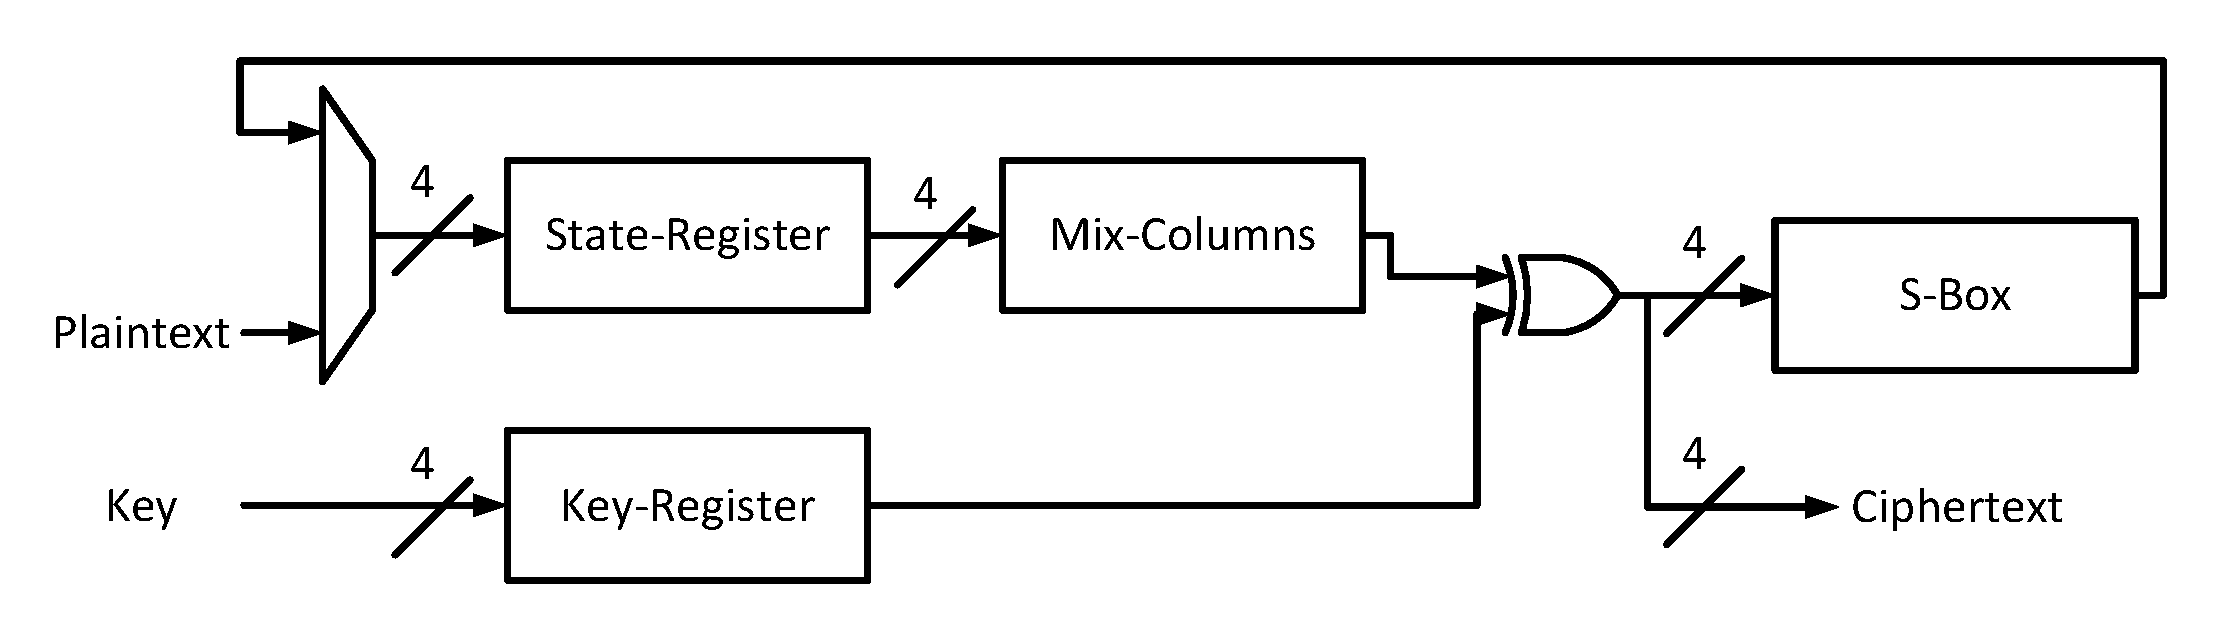
\includegraphics[width=0.7\textwidth]{./fig/serial-archticture.pdf}
    \caption{Serial architecture of CRAFT}\label{fig3}
\end{figure*}


\subsubsection{S-Box Optimization }\label{subsubsec1}


The S-Box is a crucial component of the encryption algorithm, adding to its complexity.
However, it also demands a significant amount of area.
There are several ways to implement the S-Box.
One prevalent approach is to use a lookup table (LUT), a technique described by Lara-Nino et al. \cite{LaraNino2017}.
This approach, while effective, requires many flip-flops, which can lead to a substantial increase in area consumption.
An alternative method is to use the logical equivalent expression of the S-Box.
This method, suggested by Bao et al. \cite{bao2019peigen} and Feng et al. \cite{Feng2023}, can help reduce area consumption.

Boolean satisfiability (SAT) solvers can be used to find S-Boxes that meet specific implementation requirements, such as meet to certain software or hardware implementation requirements.
To elaborate, the S-Box implementation can be encoded as Boolean constraints.
This is done by representing the S-Box as a truth table and using Boolean variables to denote the input and output bits of the S-Box.
The constraints are then formulated based on the desired properties of the S-Box.
Once the S-Box properties are encoded as Boolean constraints, these constraints can be satisfied by a SAT solver.
This assignment corresponds to an S-Box that fulfills the desired properties.

A measure of the number of logical gates required to implement the Boolean formula that represents a SAT instance is the Gate Equivalent Complexity (GEC).
To calculate the GEC, the Boolean formula is converted into a circuit of logical gates, such as AND, OR, and NOT gates.
The total count of these gates in the circuit gives the GEC of the instance.
In this design, the GEC encoding scheme from Feng et al. \cite{Feng2023} is optimized and used to implement the S-Box.
The encoding scheme is detailed in Equations~\ref{eq1}:



% \begin{align*}
% \begin{split}

\begin{flalign}
    \forall i \in & \{0,1,\ldots ,K-1\}: \nonumber                                                                        \\
    T_i =         & F_{if} (GT_i[0], \thicksim (X_{4i} \cdot X_{4i+1}) \cdot \thicksim X_{4i+2} \cdot X_{4i+3}) \nonumber \\
                  & + F_{if} (GT_i[1], X_{4i+2} \cdot (X_{4i} + X_{4i+1})) \nonumber                                      \\
                  & + F_{if} (GT_i[2], X_{4i} \cdot X_{4i+1} \cdot X_{4i+2})  \label{eq1}                                 \\
                  & + F_{if} (GT_i[3], X_{4i+2}) + F_{if} (GT_i[4], X_{4i}) \nonumber                                     \\
                  & + F_{if} (GT_i[5], X_{4i} \cdot X_{4i+1}) \nonumber                                                   \\
                  & + F_{if} (GT_i[6], X_{4i} + X_{4i+1}) + F_{if} (GT_i[7], max) \nonumber
\end{flalign}



where $K$ is numbers of the logical gates, $X_{4i}-X_{4i+3}$ is the input of the $i^{th}$ logical gate, $T_i$ is the output of the $i^{th}$ logical gate, and $F_{if}$ is a function that returns the value of the second argument if the first argument is true and returns the value of zero otherwise.
The value of $max$ is all one's in the binary expression, which is represented logically as an inverse.
$GT_i$ denotes the type of the $i^{th}$ logical gate, represented as an 8-bit binary number. The least significant bit of $GT_i$ is indexed at seven.
Table~\ref{tab3} enumerates the various types of logical gates employed in this encoding scheme.


Equations~\ref{eq2} display the optimized scheme of the S-Box, where $X_3-X_0$ represents the input and $Y_3-Y_0$ represents the output.
The proposed S-Box scheme is implemented using four MOAI1 gates, three MAOI1 gates, and one AND3 gate.
This configuration of the S-Box module results in a 28.9\% reduction in area compared to the method proposed by Bao et al. \cite{bao2019peigen}, based on gate equivalent (GE) estimation using the UMC 180nm library.

\begin{align}
    T_0 & = \text{MAOI1}(X_0, X_1, X_0, X_1) \nonumber            \\
    T_1 & = \text{AND3}(X_3, X_2, X_3) \nonumber                  \\
    T_2 & = \text{MAOI1}(X_1, X_2, X_0, X_3) \nonumber            \\
    T_3 & = \text{MOAI1}(X_1, X_0, X_2, X_2) \nonumber            \\
    T_4 & = \text{MOAI1}(X_3, T_0, T_3, T_3) \label{eq2}          \\
    T_5 & = \text{MOAI1}(T_3, T_0, X_0, T_1) \nonumber            \\
    T_6 & = \text{MAOI1}(X_0, T_0, X_3, T_0) \nonumber            \\
    T_7 & = \text{MOAI1}(X_0, T_1, T_2, T_2) \nonumber            \\
    Y_3 & = T_4 \quad Y_2 = T_6 \quad Y_1 = T_7 \quad  Y_0  = T_5
    \nonumber
\end{align}


\begin{table}[h]
    \caption{Encoding of different types of logical gates}\label{tab3}%
    \begin{tabular}{|c|c|c|}
        \hline
        logical expression                                   & $GT_i$ & gate type \\
        \hline
        $X_0 \oplus X_1$                                     & 2      & XOR       \\
        $\sim (X_0 \oplus X_1)$                              & 3      & XNOR      \\
        $X_0 \land X_1$                                      & 4      & AND       \\
        $\sim (X_0 \land X_1)$                               & 5      & NAND      \\
        $X_0 \lor X_1$                                       & 6      & OR        \\
        $\sim (X_0 \lor X_1)$                                & 7      & NOR       \\
        $\sim X_0$                                           & 9      & NOT       \\
        $\sim X_1$                                           & 11     & NOT       \\
        $\sim X_2$                                           & 17     & NOT       \\
        $X_0 \oplus X_1 \oplus X_2$                          & 18     & XOR3      \\
        $\sim (X_0 \oplus X_1 \oplus X_2)$                   & 19     & XNOR3     \\
        $X_0 \land X_1 \land X_2$                            & 32     & AND3      \\
        $\sim (X_0 \land X_1 \land X_2)$                     & 33     & NAND3     \\
        $X_0 \lor X_1 \lor X_2$                              & 118    & OR3       \\
        $\sim (X_0 \lor X_1 \lor X_2)$                       & 119    & NOR3      \\
        $\sim ((X_0 \land X_1) \lor (\sim (X_2 \lor X_3)))$  & 176    & MAOI1     \\
        $\sim (\sim (X_0 \land X_1) \land ((X_2 \lor X_3)))$ & 177    & MOAI1     \\
        \hline
    \end{tabular}
\end{table}

\subsubsection{Mix-Columns Optimization}\label{subsubsec2}

The Mix-Columns component is a linear transformation of the input column.
The output column is generated by multiplying the input column with a constant matrix $M$.
$M$ is a involutory matrix, which means $M^2 = E$, where $E$ is the identity matrix.
It is easy to decrypt the ciphertext by multiplying the ciphertext with $M$ again.
Equation~\ref{eq3} illustrates the Mix-columns component.
Here, $I_{3,j}$, $I_{2,j}$, $I_{1,j}$, and $I_{0,j}$ represent the input column, while $I'_{3,j}$, $I'_{2,j}$, $I'_{1,j}$, and $I'_{0,j}$ denote the output column.
The column index is given by $j$, where $j$ ranges from 0 to 3.

\begin{equation}
    \begin{bmatrix}
        I'_{3,j} \\
        I'_{2,j} \\
        I'_{1,j} \\
        I'_{0,j}
    \end{bmatrix}
    =
    \begin{bmatrix}
        1 & 0 & 0 & 0 \\
        0 & 1 & 0 & 0 \\
        1 & 0 & 1 & 0 \\
        1 & 1 & 0 & 1
    \end{bmatrix}
    \begin{bmatrix}
        I_{3,j} \\
        I_{2,j} \\
        I_{1,j} \\
        I_{0,j}
    \end{bmatrix}
    \label{eq3}
\end{equation}


In order to reduce the area of this component, the serial architecture of Mix-Columns is utilized, as shown in Figure~\ref{serial_mix_columns_fig}.
The serial architecture of Mix-Columns requires four 4-bit registers, two multiplexers, and three XOR gates.
The operation of Mix-Columns involves three distinct stages: freeze, shift, and add.
During the freeze stage, the register values are kept unchanged by setting both $CM_0$ and $CM_1$ to 0.
In the shift stage, a shift in the register values from $RM_0$ to $RM_4$ is induced by setting both $CM_0$ and $CM_1$ to 1.
Finally, in the add stage, an addition operation on the column values is executed according to Equation~\ref{eq3}. This is achieved by setting $CM_0$ and $CM_1$ to 0 and 1, respectively.

Figure~\ref{serial_time_diagrm_mix_colunms} presents the timing diagram for the serial architecture of the Mix-Columns operation.
It requires five clock cycles to compute the next columns from the previous ones, and an additional four clock cycles to transfer data from the internal register of Mix-Columns to the State-Register.
Therefore, a complete state round requires a total of 36 clock cycles.


\begin{figure}[h]%   
    \centering
    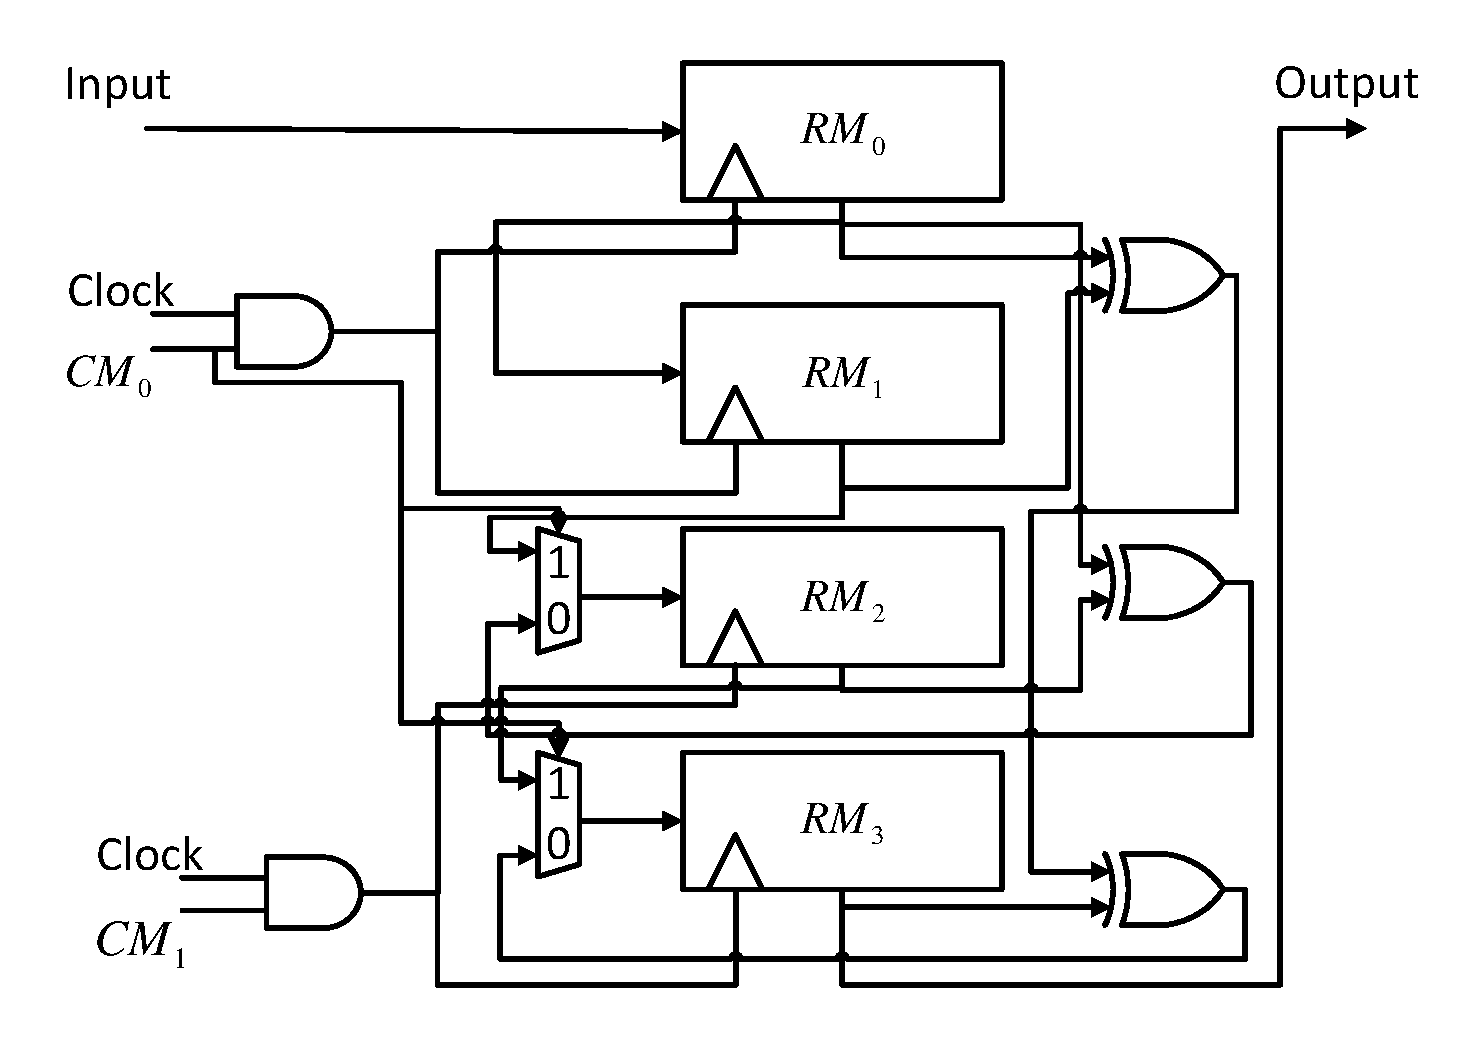
\includegraphics[width=0.45\textwidth]{./fig/Mix-Columns.pdf}
    \caption{Serial Architecture of Mix-Columns with clock gating}\label{serial_mix_columns_fig}
\end{figure}

\begin{figure}[h]%   
    \centering
    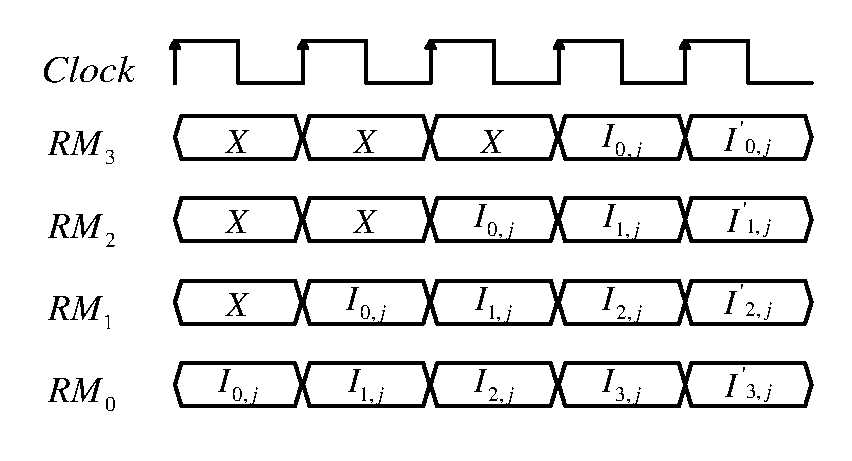
\includegraphics[width=0.45\textwidth]{./fig/Mix-Columns-Times.pdf}
    \caption{Timing Diagram for the Serial Architecture of Mix-Columns }
    \label{serial_time_diagrm_mix_colunms}
\end{figure}

\subsubsection{Control Units}\label{subsubsec3}

As depicted in Figure~\ref{serial_fsm_fig}, the finite-state machine (FSM) initiates the encryption process by loading the initial key into the Key-Register and the plaintext into the State-Register.
During the Key-Schedule phase, the key is expanded while the gate clocks of the Mix-Columns and State-Register are turned off.
Next, the Mix-Columns phase begins, where one column of the State-Register is stored in the Mix-Columns registers. 
The Mix-Columns operation on one column takes five clock cycles to execute in this phase.
Once this phase is finished, the gate clocks for the State-Register and Key-Register are turned off.
Following this, the Sub-Box phase commences. 
During this phase, the data from the Mix-Columns registers is transferred again to the State-Register and XORed with the keys.
This process requires an additional four clock cycles.
This cycle between the Mix-Columns and Sub-Box phases is repeated four times for the four columns of the State-Register.
Subsequently, the Permute operation is carried out within the State-Register, requiring a single clock cycle.
The encryption process concludes when the Round counter reaches 31, at which point the ciphertext is stored in the State-Register.

\begin{figure}[h]%   
    \centering
    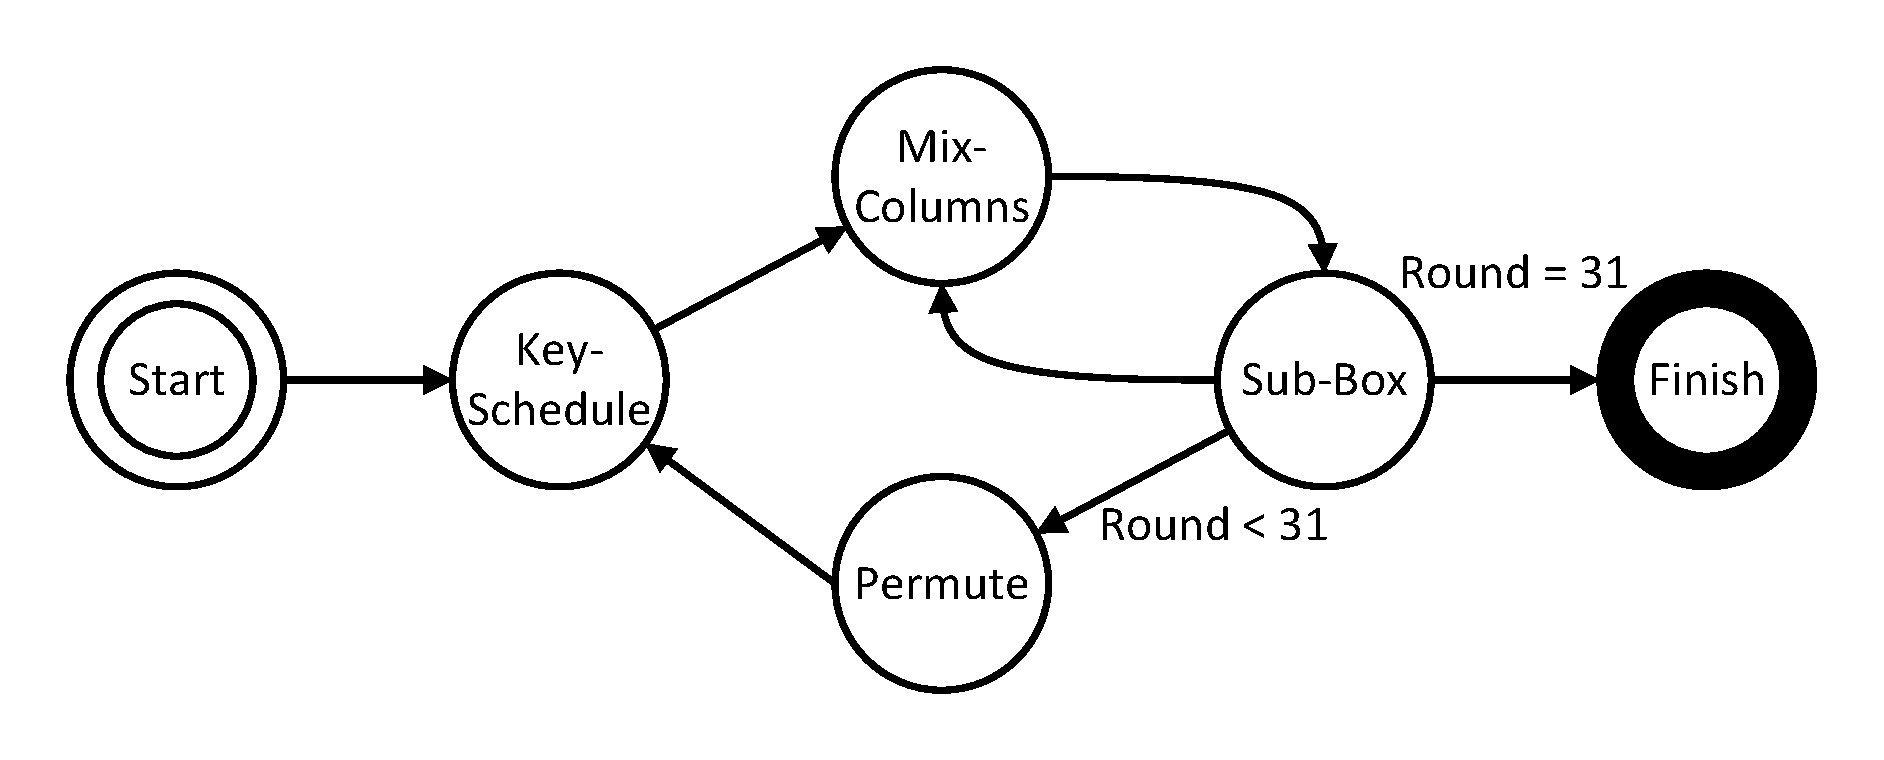
\includegraphics[width=0.45\textwidth]{./fig/serial-fsm.pdf}
    \caption{Finite-state machine for Serial Architecture}\label{serial_fsm_fig}
\end{figure}

In the work of Shahbazi et al. \cite{Shahbazi2021}, it is discussed that the dynamic power consumption of the encryption process can be mitigated through the use of clock gating.
The clock gating technique is independently applied to the State-Register, Key-Register, and Mix-Columns.
For instance, in the Permute phase, the gate clocks of the Key-Register and Mix-Columns are disabled as these components are not in use.
This helps save a significant amount of power. Figure~\ref{serial_time_diagrm} shows the timing diagram of a design that uses the clock gating technique.

\begin{figure}[h]%   
    \centering
    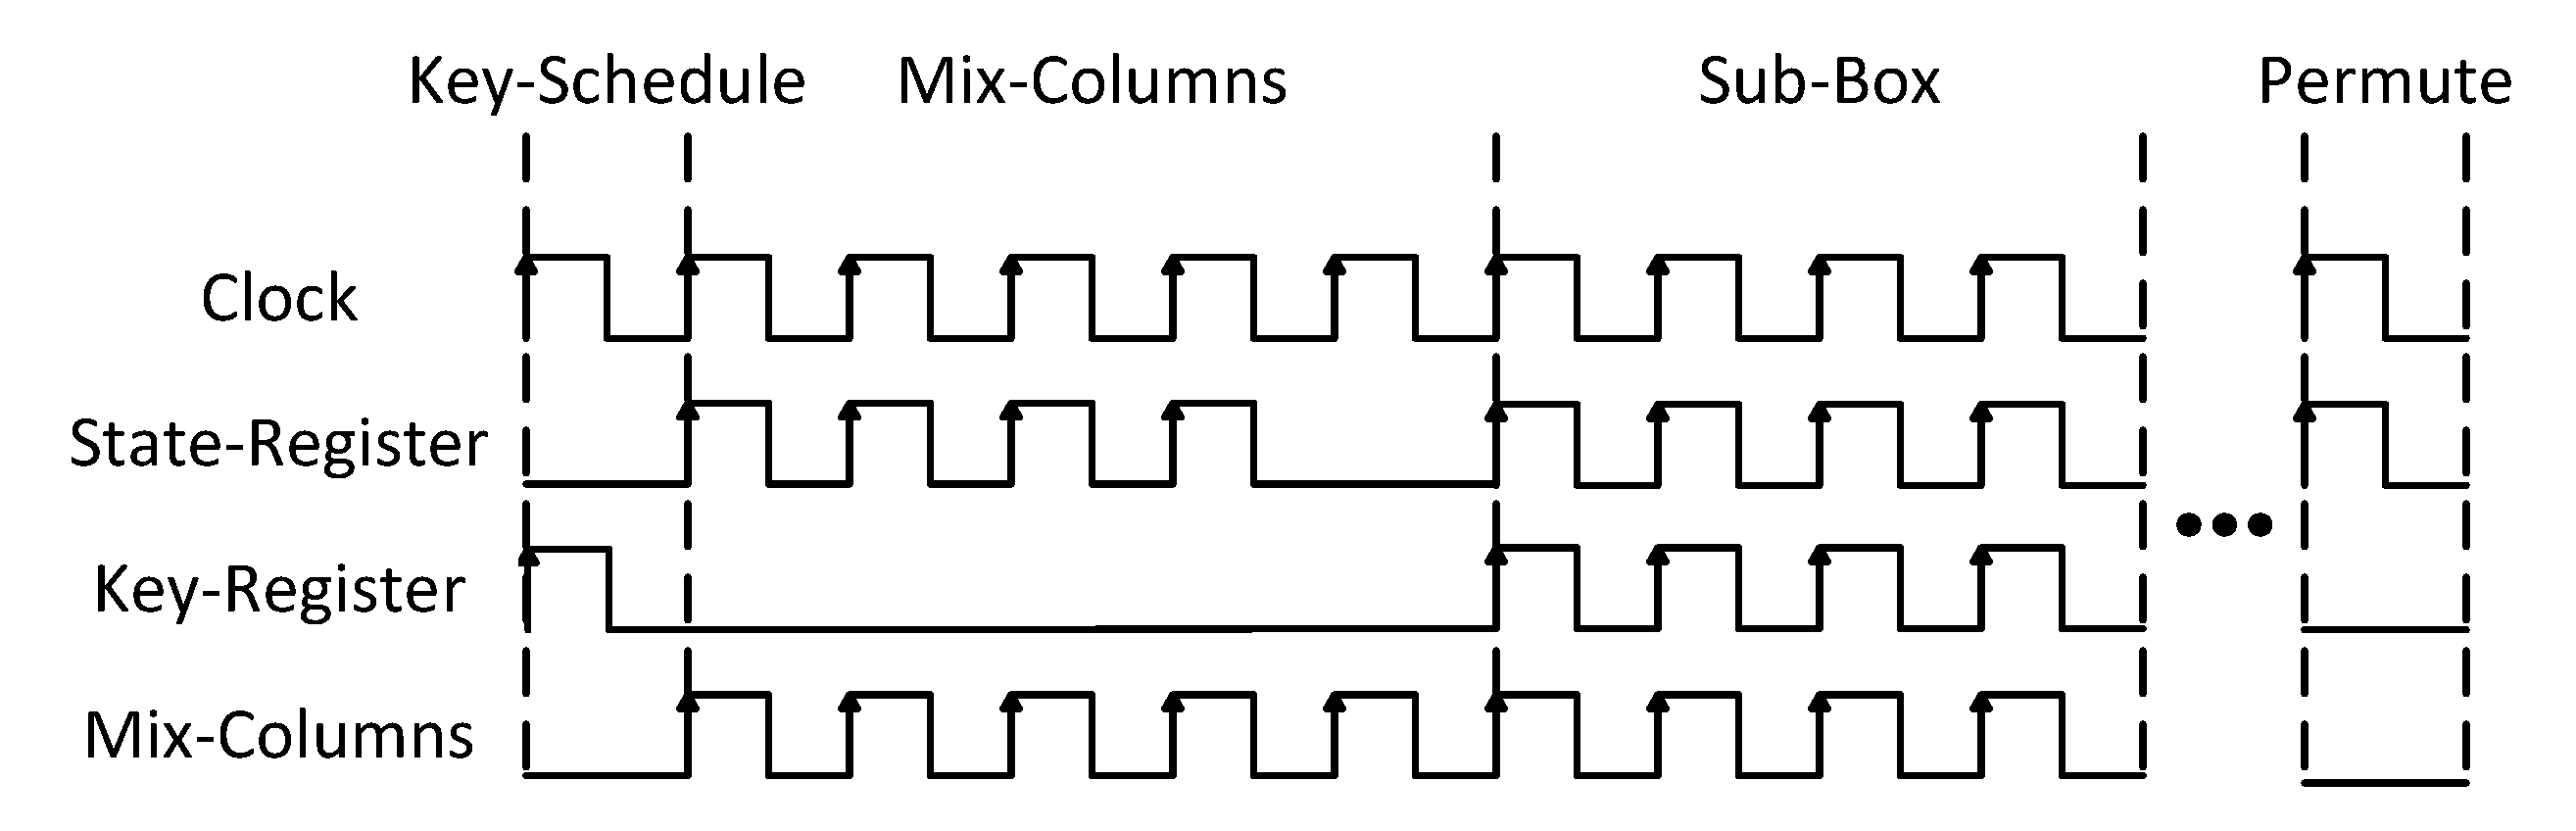
\includegraphics[width=0.45\textwidth]{./fig/serial-time.pdf}
    \caption{Timing diagram for Serial Architecture}\label{serial_time_diagrm}
\end{figure}
\subsection{Unrolled Architecture (UA)}\label{subsec3}

The unrolled architecture shown in Figure~\ref{fig4} includes two Sub-Boxes, two Mix-Columns, a Key, a State-Register, two PermuteNibbles, and one feedback path. It's designed to perform a 30-round encryption process in just 15 cycles. Only the Mix-Columns and Add-Key operations are carried out in the final cycle, finishing the encryption process in a total of 16 cycles.

The unrolled architecture, which is based on the iterative architecture from the work of Beierle et al. \cite{Beierle2019}, completes the encryption process in only 16 cycles, compared to the 32 cycles needed by the iterative architecture. Here, a cycle includes two round functions of CRAFT. While this approach might use more area, it provides higher throughput at the same frequency.


\begin{figure*}[h]%   
    \centering
    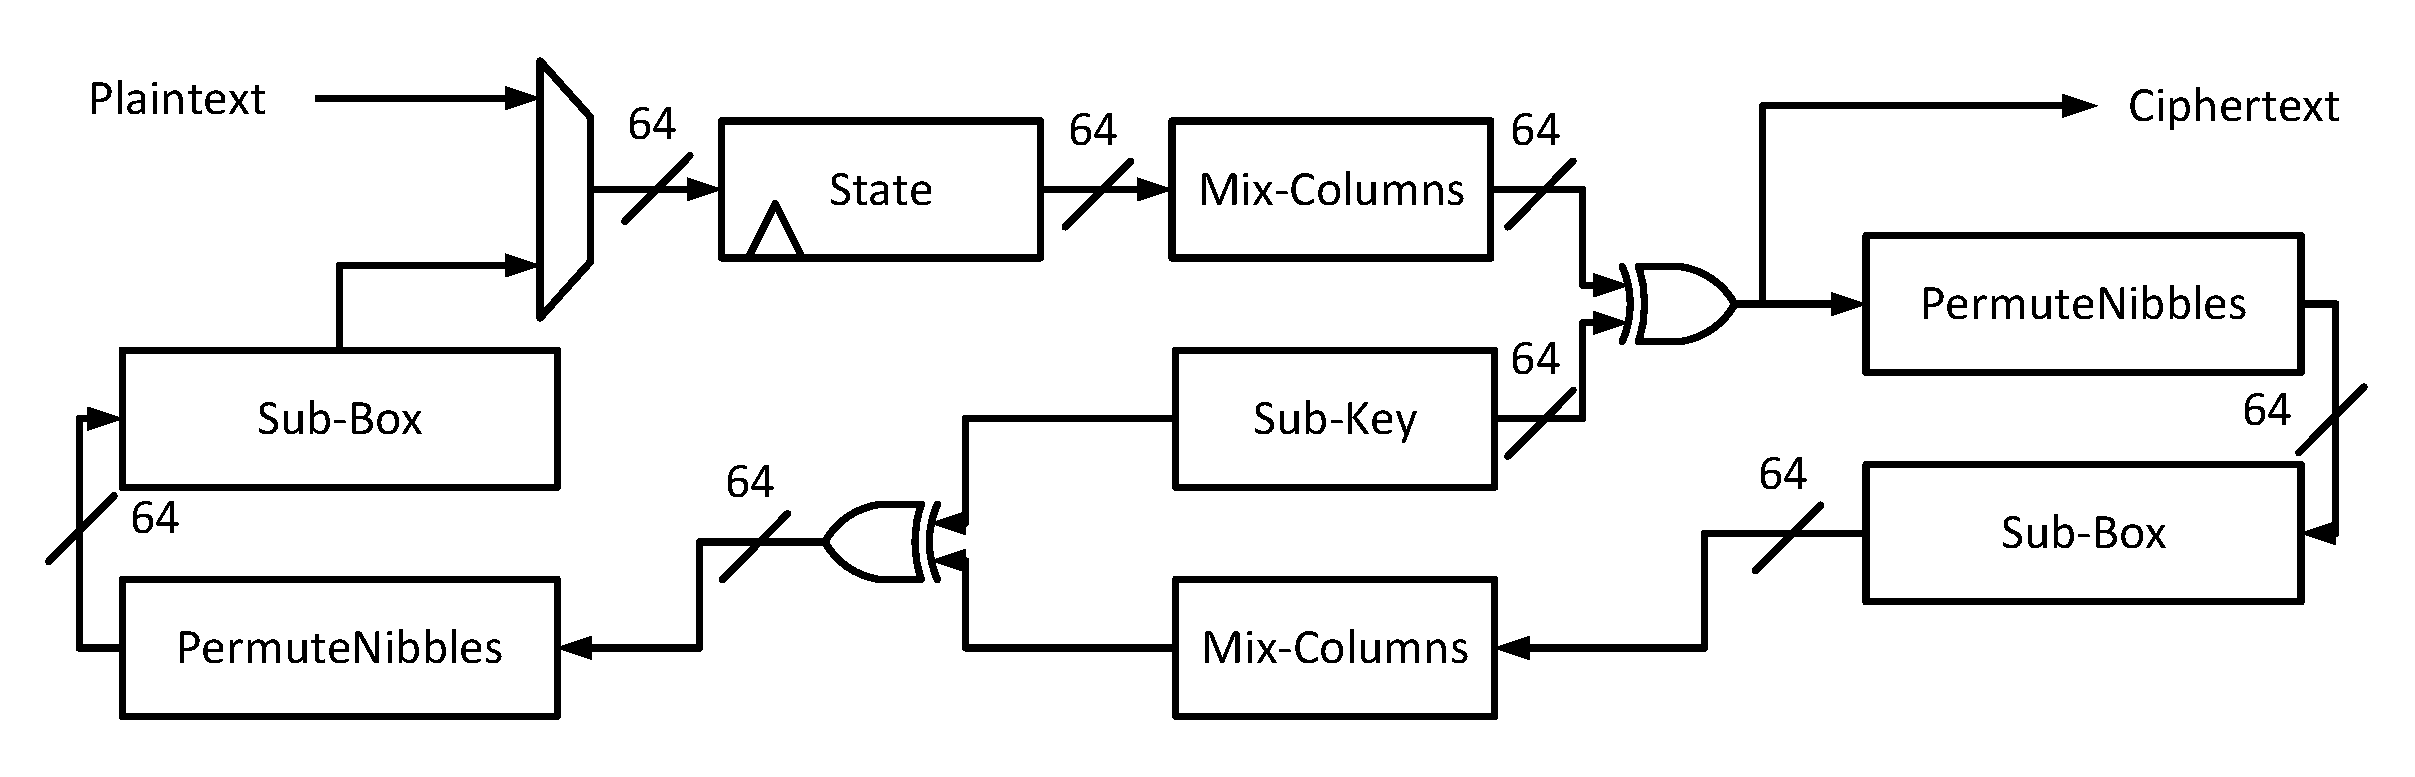
\includegraphics[width=0.7\textwidth]{./fig/unrolled-archticture.pdf}
    \caption{Unrolled architecture of CRAFT}\label{fig4}
\end{figure*}

\subsection{Iterative Architecture (IA)}\label{iterative_architecture}

The architecture proposed by Bharathi et al. \cite{Bharathi2022} operates on a round-based architecture.
It employs a single round function to encrypt a block, incorporating a Sub-Box, a Permute, and an Add-Key operation.
This round function is executed 32 times to encrypt a single block. Simultaneously, the Key Schedule operates in parallel with the round function. This architecture is illustrated in Figure~\ref{fig5}.
For comparison, different architectures are listed in Table~\ref{tab2}.

\begin{figure*}
    \centering
    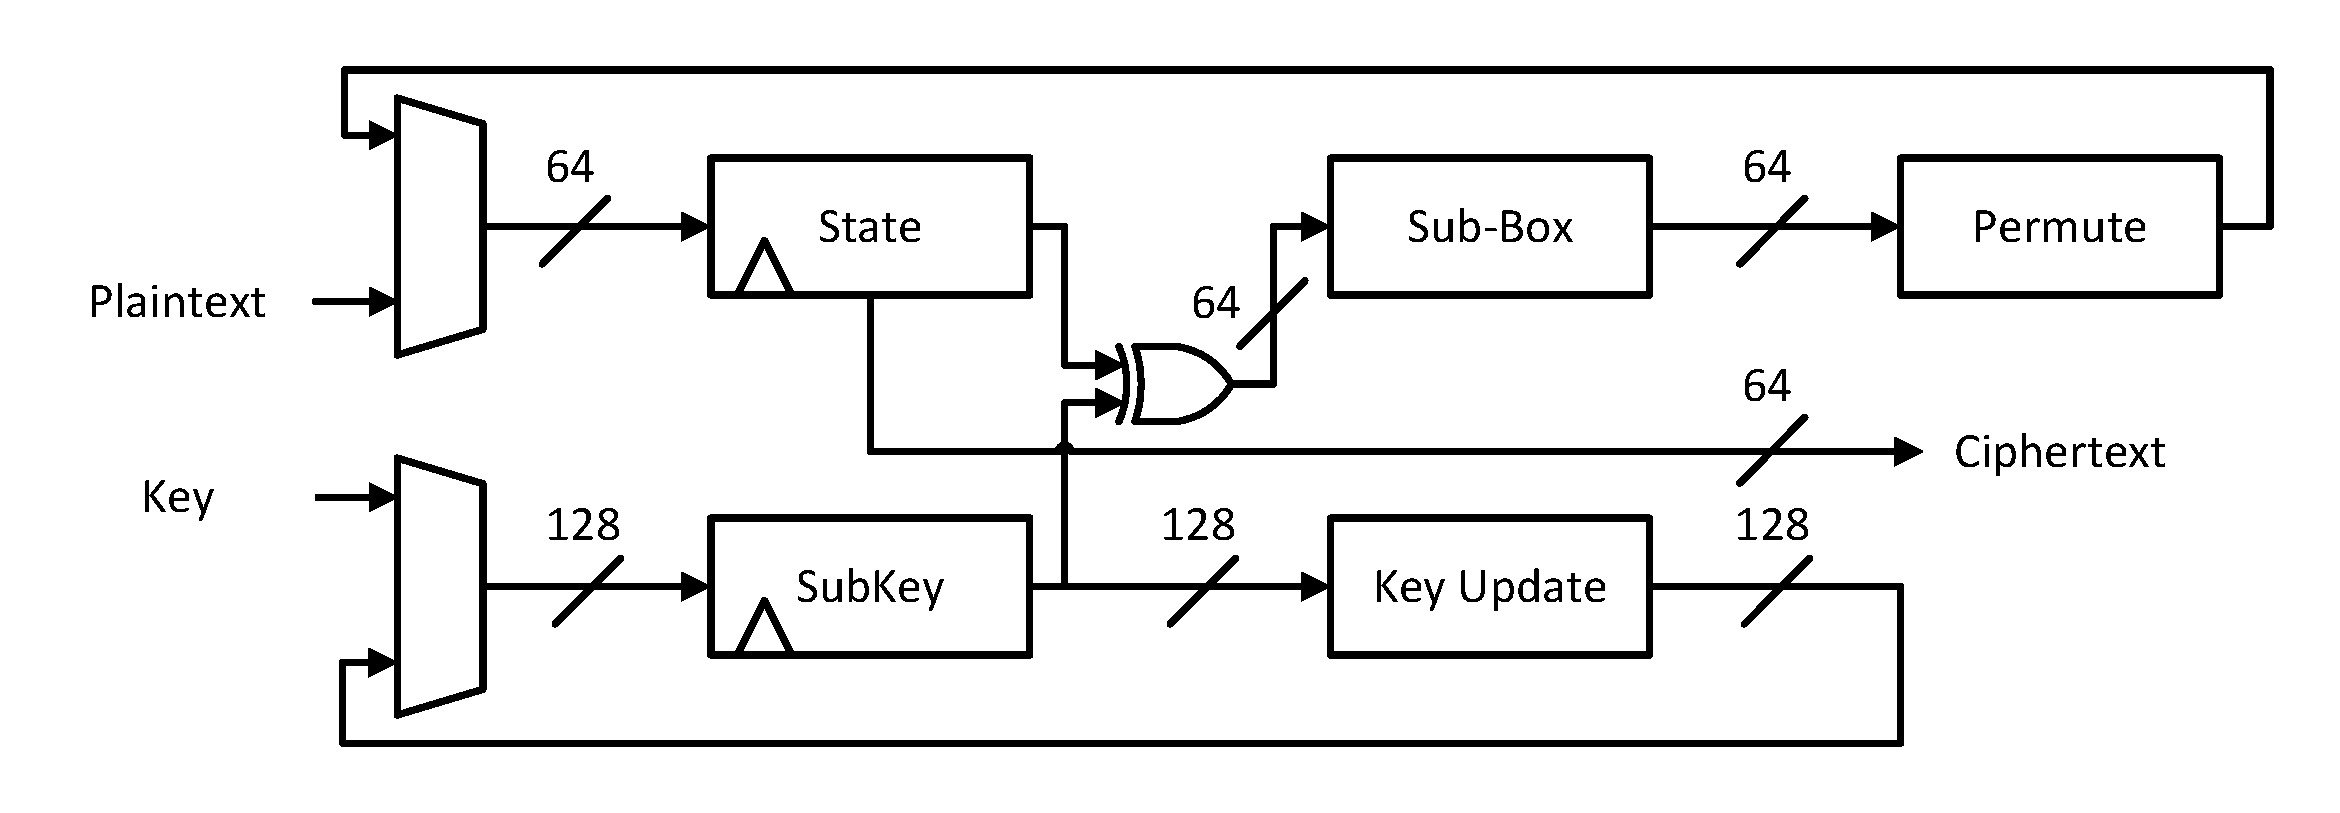
\includegraphics[width=0.75\textwidth]{./fig/iteration-present.pdf}
    \caption{Iterative architecture of PRESENT}\label{fig5}
\end{figure*}

\begin{table}[h]
    \centering
    \caption{Description of Different Architectures}\label{tab2}%
    \begin{tabular}{|c|c|c|c|}
        \hline
        Architecture & Cipher  & Description & Reference           \\
        \hline
        SA           & CRAFT   & Serial      & This work           \\
        UA           & CRAFT   & Unrolled    & This work           \\
        IA           & PRESENT & Iterative   & \cite{Bharathi2022} \\
        \hline
    \end{tabular}
\end{table}


\section{Experimental Evaluation}\label{sec4}

In ASIC implementations, the Gate Equivalent (GE) is often used to evaluate the area consumption of a design.
One GE corresponds to the area of a two-input NAND gate. 
The area is computed in terms of GEs. 
This is done by dividing the total area (measured in $\mu m^2$) by the area of a two-input NAND gate (also measured in $\mu m^2$).
However, the number of GEs can vary depending on the specific technology used, as Turan et al. discuss in their work \cite{Turan}.
For instance, the number of GEs for the same design will differ between UMC 180nm technology and TSMC 180nm technology.
Therefore, GE is not suitable for comparing the area consumption of different designs on different technologies.
For a fair comparison, the area consumption of the proposed designs is assessed using FPGA implementations.
This is a technique similarly employed in the study by Mohajerani et al. \cite{Mohajerani2020}.

\subsection{Platform}\label{subsec4}

The designs proposed in this study were implemented on a Xilinx FPGA board, utilizing the Vivado v2023.2 software for deployment.
Benchmarking was performed across three distinct FPGA platforms to ensure a diverse testing environment: Artix-7(xc7a100tcsg324-1), Kintex-7(xc7k70tfbg484-1), and Spartan-7(xc7s100fgga484-1).
Artix-7 offers high performance in resource-limited situations. Spartan-7 is designed for high-restriction environments. Kintex-7 is well-suited for use in applications such as 3G and 4G wireless technologies.


\subsection{Area}\label{subsec5}

The area consumed by the proposed designs is quantified using the Area metric, which encompasses components such as Flip-Flops, LUTs, and Slices.
For a balanced comparison, the embedded memory blocks of the FPGA were not utilized.
This was achieved by disabling the relevant settings in the VHDL, as recommended in the design guidelines provided by Xilinx \cite{xilinx2022ultrafast}.
Also, all designs were synthesized and implemented using the same settings, specifically, the default settings of Vivado Synthesis and Implementation.

\subsection{Throughput}\label{subsec6}
The efficiency of the proposed designs is assessed using the Throughput metric.
This metric uses three parameters: the maximum throughput rate, the throughput rate at 100MHz, and the throughput rate per slice.
The maximum throughput rate is the highest rate that our designs can achieve, calculated using Equation~\ref{eq4}.
The throughput rate at 100MHz shows the rate achievable when the clock frequency is set to 100MHz, calculated using Equation~\ref{eq5}.
The throughput rate per slice is a measure of efficiency, calculated by dividing the throughput rate by the number of Slices, as defined in Equation~\ref{eq6}.
In these computations, the Plaintext Size is set to 64-bit.
Latency denotes the count of clock cycles needed to encrypt a single block, and Slices represent the quantity of Slices consumed by the design.
\begin{equation}
    MaxThroughput(Thr) = \frac{MaxFrequency \times Block Size}{Latency}
    \label{eq4}
\end{equation}

\begin{equation}
    Throughput_{@100MHz}(Thr^*) = \frac{100MHz \times Block Size}{Latency}
    \label{eq5}
\end{equation}

\begin{equation}
    ThroughputPerSlice = \frac{Thr}{Slices}
    \label{eq6}
\end{equation}

\subsection{Power and Energy}\label{power_energy}

The Power metric, which includes both dynamic and static power consumption, is used to evaluate the power consumption of the proposed designs, as defined in Equation~\ref{eq7}.
On the other hand, the Energy metric measures the energy consumption of the designs. It's calculated by multiplying the power consumption by the time needed to encrypt a single block. This time is determined by dividing the latency by the frequency, as explained in Equation~\ref{enery_eqation}.

\begin{align}
    \text{Total Power} (TP) & = \text{Dynamic Power} (DP) \nonumber \\
                            & + \text{Static Power} (SP)
    \label{eq7}
\end{align}
\begin{equation}
    Energy(E) = \frac{TP \times Latency }{Frequency}
    \label{enery_eqation}
\end{equation}


\section{Results}\label{sec5}

This section details the outcomes of the proposed designs, categorized into three aspects: area consumption, throughput performance, and power and energy metrics.
The results are demonstrated across three different FPGA platforms: Artix-7, Kintex-7, and Spartan-7.
The area consumption of the designs is presented in Table~\ref{area_compare}. The throughput results can be found in Table~\ref{throughput_compare}, and the details of power and energy consumption are provided in Table~\ref{power_energy_compare}.


\begin{table*}[h]
    \caption{Area Used in Three Architectures}\label{area_compare}%
    \begin{tabular*}{\textwidth}{@{\extracolsep\fill}|c|c|c|c|c|c|c|}
        \hline
        Platform & Design & $State(bit)$ & $Key(bit)$ & $FF$ & $LUT$ & $Slices$ \\
        \hline
        \multirow{3}{*}{Artix-7}  & SA & 64 & 128 & \textbf{144} & \textbf{177} & \textbf{59} \\
        & UA & 64 & 128 & 157 & 378 & 111 \\
        & IA & 64 & 128 & 201 & 243 & 70 \\
        \hline
        \multirow{3}{*}{Kintex-7} & SA & 64 & 128 & \textbf{144} & \textbf{178} & \textbf{58}\\
        & UA & 64 & 128 & 157 & 377 & 115 \\
        & IA & 64 & 128 & 201 & 244 & 68 \\
        \hline
        \multirow{3}{*}{Spartan-7} & SA & 64 & 128 & \textbf{144} & \textbf{177} & \textbf{57}\\
        & UA & 64 & 128 & 157 & 381 & 118 \\
        & IA & 64 & 128 & 201 & 244 & 70 \\
        \hline
    \end{tabular*}
\end{table*}

\begin{table*}
    \begin{threeparttable}
        \caption{Throughput Results in Three Architectures}\label{throughput_compare}%
        \begin{tabular*}{\textwidth}{@{\extracolsep\fill}|c|c|c|c|c|c|c|}
            \hline
            Platform & Design & $Latency$ & $MaxF(MHz)$ & $Thr(Mbps)$ & $Thr^*(Mbps)$\tnote{a} & $Thr/Slices$($Kbps/Slices$) \\
            \hline
            \multirow{3}{*}{Artix-7}  & SA & 1215 & \textbf{557.41} & 29.36 & 5.27 & 497.65 \\
            & UA & \textbf{16} & 142.38 & 569.52 & \textbf{400.00} & 5130.81 \\
            & IA & 32 & 274.04 & 548.08 & 200.00 & 7829.71 \\
            \hline
            \multirow{3}{*}{Kintex-7} & SA & 1215 & \textbf{853.97} & 44.98 & 5.27 & 775.57 \\
            & UA & \textbf{16} & 175.25 & 701.00 & \textbf{400.00} & 6095.65 \\
            & IA & 32 & 357.78 & 715.56 & 200.00 & 10522.94 \\
            \hline
            \multirow{3}{*}{Spartan-7} & SA & 1215 & \textbf{525.76} & 27.69 & 5.27 & 485.87 \\
            & UA & \textbf{16} & 138.86 & 555.44 & \textbf{400.00} & 4707.12 \\
            & IA & 32 & 296.29 & 592.58 & 200.00 & 8465.43 \\
            \hline
        \end{tabular*}
        \begin{tablenotes}
            \item[a] Throughput rate at 100MHz
        \end{tablenotes}
    \end{threeparttable}
\end{table*}

\begin{table*}
    \begin{threeparttable}
        \caption{Power and Energy Consumption in Three Architectures}\label{power_energy_compare}%
        \begin{tabular*}{\textwidth}{@{\extracolsep\fill}|c|c|c|c|c|c|c|}
            \hline
            Platform & Design & $DP(mW)$ & $SP(mW)$ & $TP(mW)$ & $E(uJ)$ & $E/bit(nJ/bit)$ \\
            \hline
            \multirow{3}{*}{Artix-7}  & SA & 2.00 & 139.00 & 141.00 & 1.71 & 26.77 \\
            & UA & 7.00 & 139.00 & 146.00 & \textbf{0.02} & \textbf{0.37} \\
            & IA & 2.00 & 139.00 & 141.00 & 0.05 & 0.71 \\
            \hline
            \multirow{3}{*}{Kintex-7} & SA & 2.00 & 145.00 & 147.00 & 1.79 & 27.91 \\
            & UA & 8.00 & 145.00 & 153.00 & \textbf{0.02} & \textbf{0.38} \\
            & IA & 3.00 & 145.00 & 148.00 & 0.05 & 0.74 \\
            \hline
            \multirow{3}{*}{Spartan-7} & SA & 2.00 & 140.00 & 142.00 & 1.73 & 26.96 \\
            & UA & 7.00 & 140.00 & 147.00 & \textbf{0.02} & \textbf{0.37} \\
            & IA & 3.00 & 140.00 & 143.00 & 0.05 & 0.72 \\
            \hline
        \end{tabular*}
        \begin{tabular}{llll}
            DP: Dynamic Power & SP: Static Power & TP: Total Power & E: Energy
        \end{tabular}
    \end{threeparttable}
\end{table*}

The area consumption of the proposed designs is evaluated based on three factors: Flip-Flops (FF), Look-Up Tables (LUT), and Slices. These designs are compared with the iterative architecture of PRESENT, as detailed in the work of Bharathi et al. \cite{Bharathi2022}. The results indicate that the proposed serial architecture consume 15.72\% less area than the iterative architecture of PRESENT.

Regarding the FF, the key schedule of the CRAFT cipher is implemented using multiplexers. This eliminates the need for FF to store the sub-key, resulting in a lower FF count compared to other ciphers. This is a significant factor contributing to the CRAFT cipher's requirement of less than 1000 GE, which is the lowest known requirement on the IBM 130 nm ASIC library, as demonstrated in the study by Beierle et al. \cite{Beierle2019}. A comparison of FF counts is provided in Figure~\ref{compare_ff}.

\begin{figure}
    \centering
    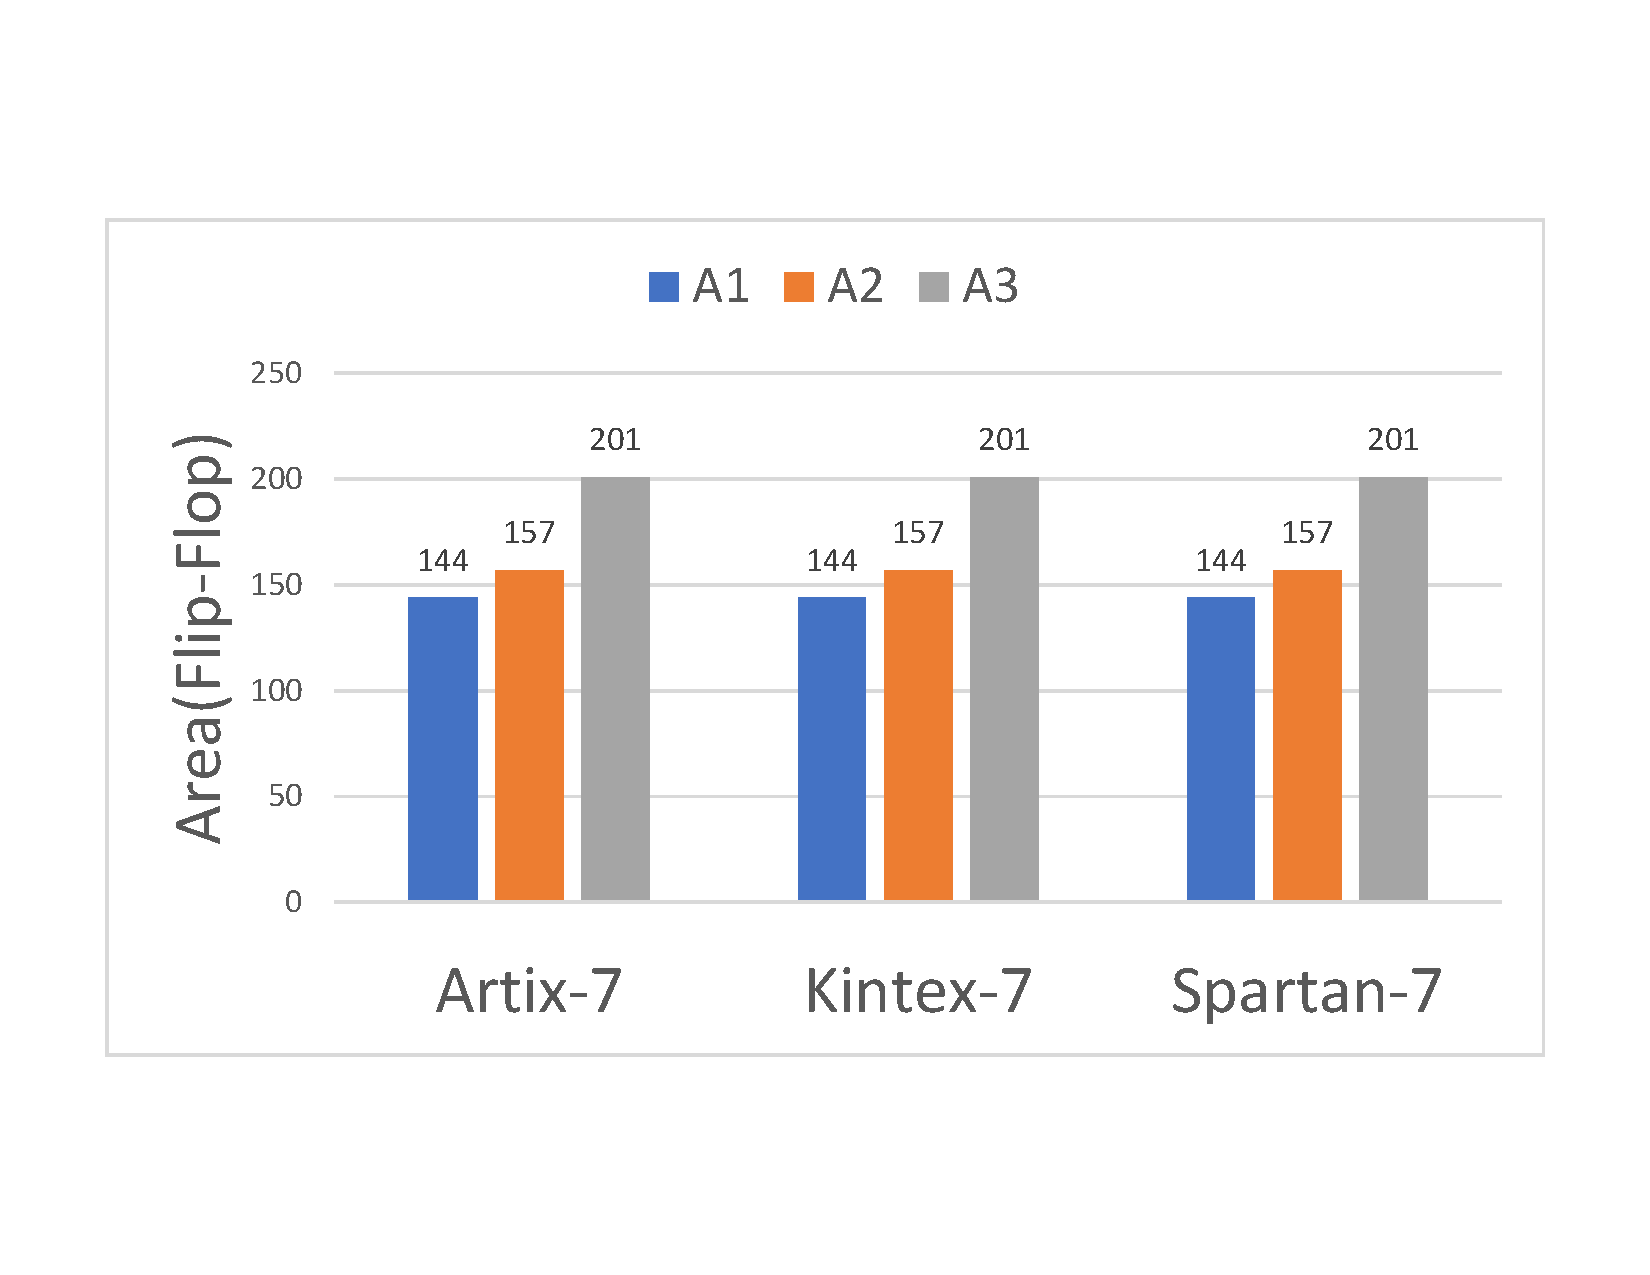
\includegraphics[width=0.45\textwidth]{./fig/compare-ff.pdf}
    \caption{Comparison of Flip-Flop in Three Architectures}\label{compare_ff}
\end{figure}

As illustrated in Figure~\ref{compare_lut}, when it comes to LUT, the proposed serial architecture require fewer LUTs than the iterative architecture of PRESENT. This is attributed to the fact that the proposed designs utilize a single S-Box, in contrast to the 16 S-Boxes used by the iterative architecture of PRESENT. Furthermore, the proposed designs also require fewer LUTs than the unrolled architecture of CRAFT, which uses 32 S-Boxes, compared to just one in the proposed designs.

\begin{figure}
    \centering
    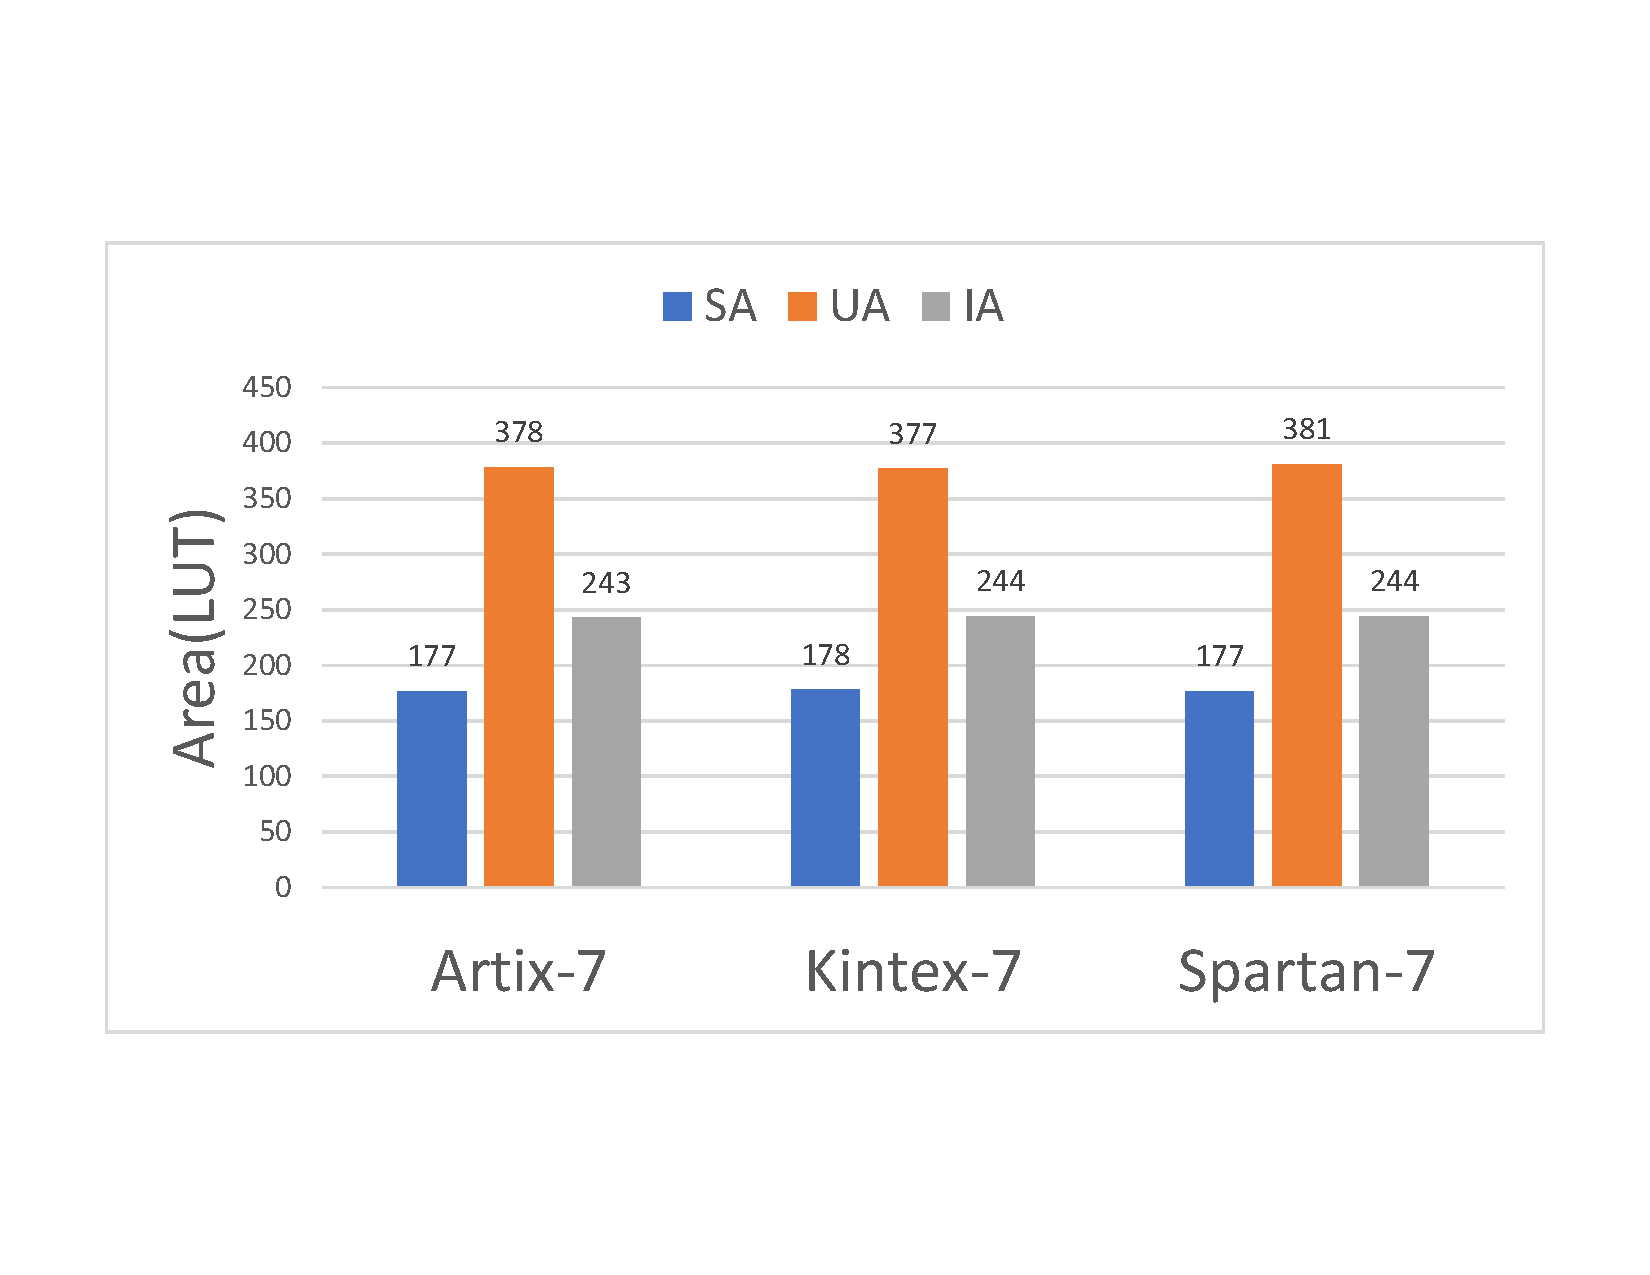
\includegraphics[width=0.45\textwidth]{./fig/compare-lut.pdf}
    \caption{Comparison of Look-Up Tables in Three Architectures}\label{compare_lut}
\end{figure}

Thanks to the reduction in Flip-Flop (FF) and Look-Up Table (LUT) usage, the serial architecture has fewer slices compared to the iterative architecture of PRESENT.
In terms of Slices efficiency, Spartan-7 outperforms both Artix-7 and Kintex-7 platforms.
These results are illustrated in Figure~\ref{compare-slices}. However, the lower Max Frequency of Spartan-7 will be considered in the Throughput comparison.

\begin{figure}
    \centering
    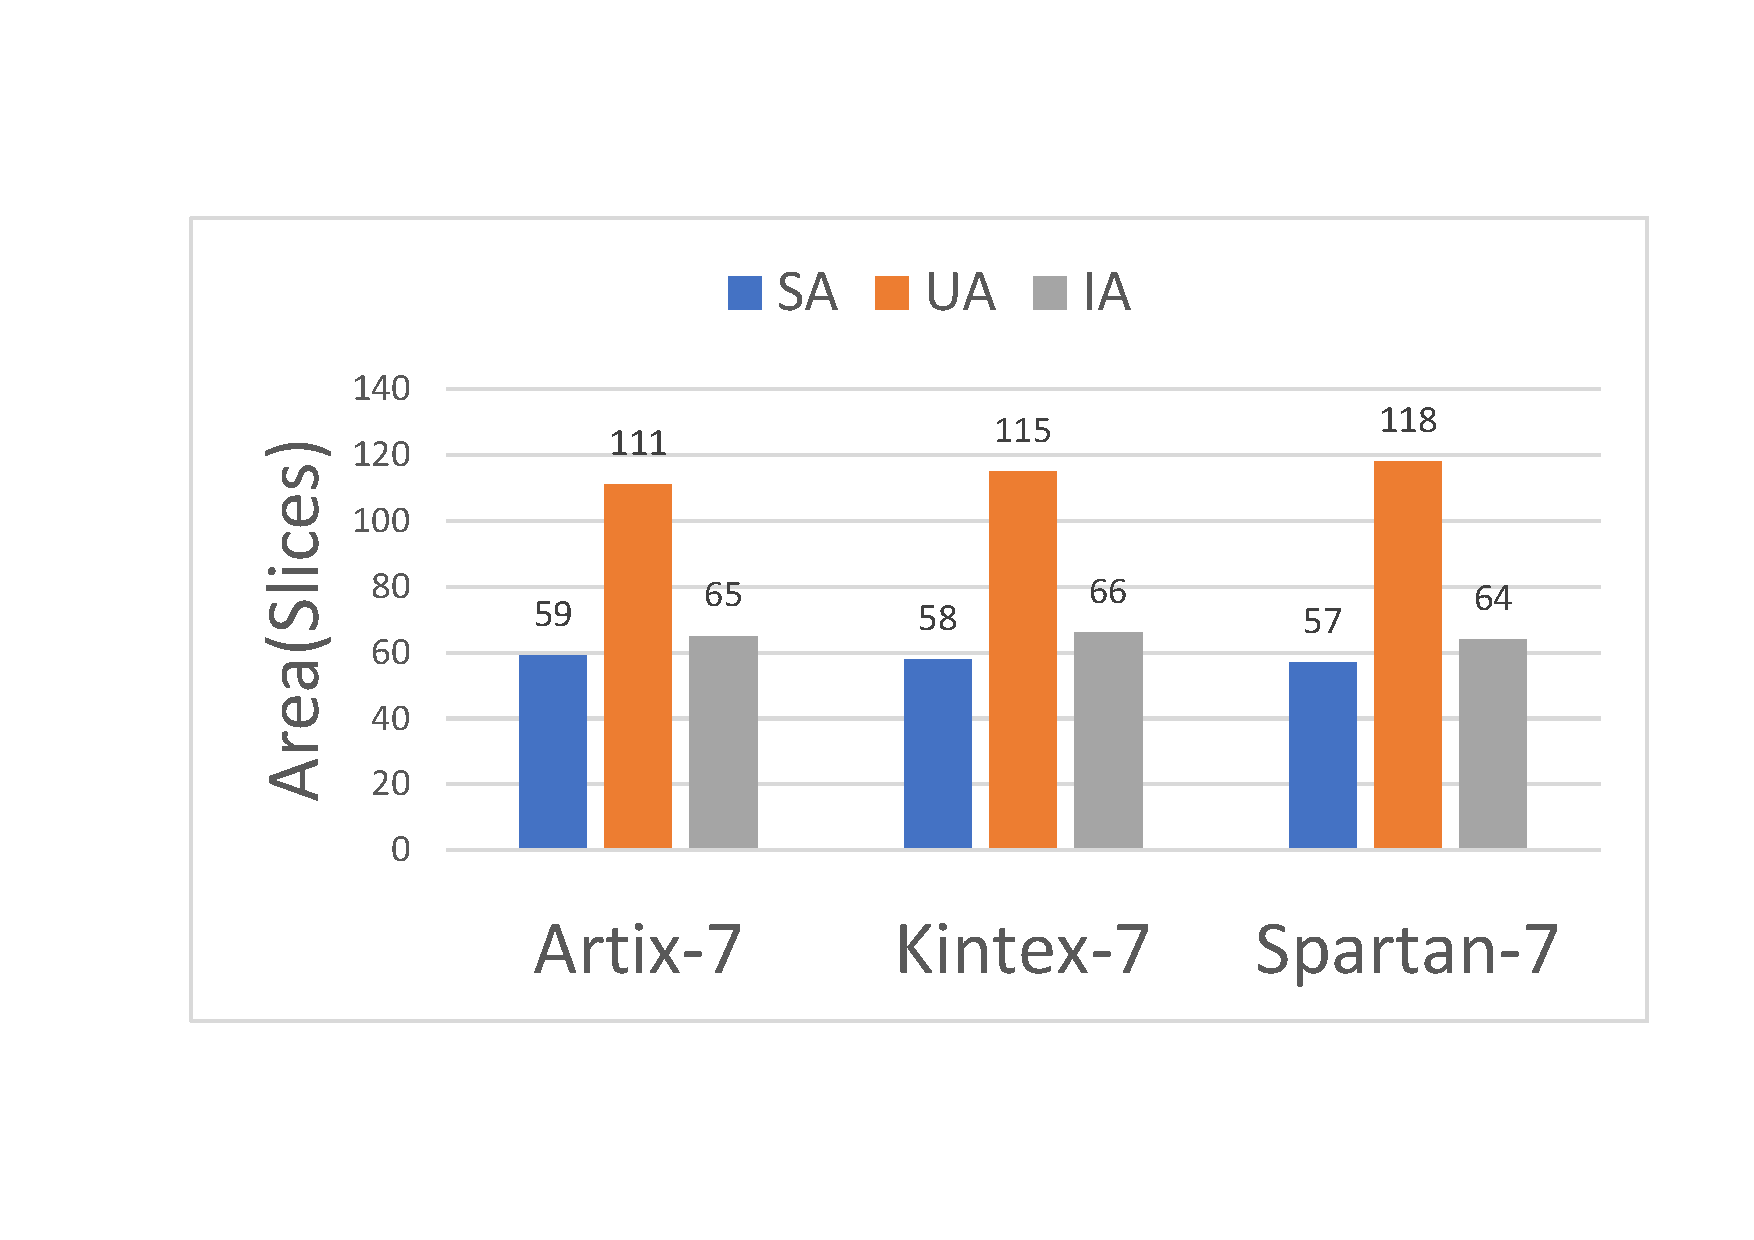
\includegraphics[width=0.45\textwidth]{./fig/compare-slices.pdf}
    \caption{Comparison of Slices in Three Architectures}\label{compare-slices}
\end{figure}

Figure~\ref{compare-maxF} illustrates that the proposed serial architecture have a higher Max Frequency than the iterative architecture of PRESENT. This improvement is due to two key factors. First, the S-Box is optimized with the GEC encoding scheme, reducing its delay. Second, the serial architecture of the design further reduces the overall delay of the encryption process. However, among all platforms, Spartan-7 has the lowest Max Frequency, primarily because it has the fewest LUTs, as shown in Figure~\ref{compare_lut}. The unrolled architecture reduces the latency to 16, which doubles the Throughput rate at 100MHz compared to the iterative architecture of PRESENT. This data is presented in Table~\ref{throughput_compare}.

\begin{figure}
    \centering
    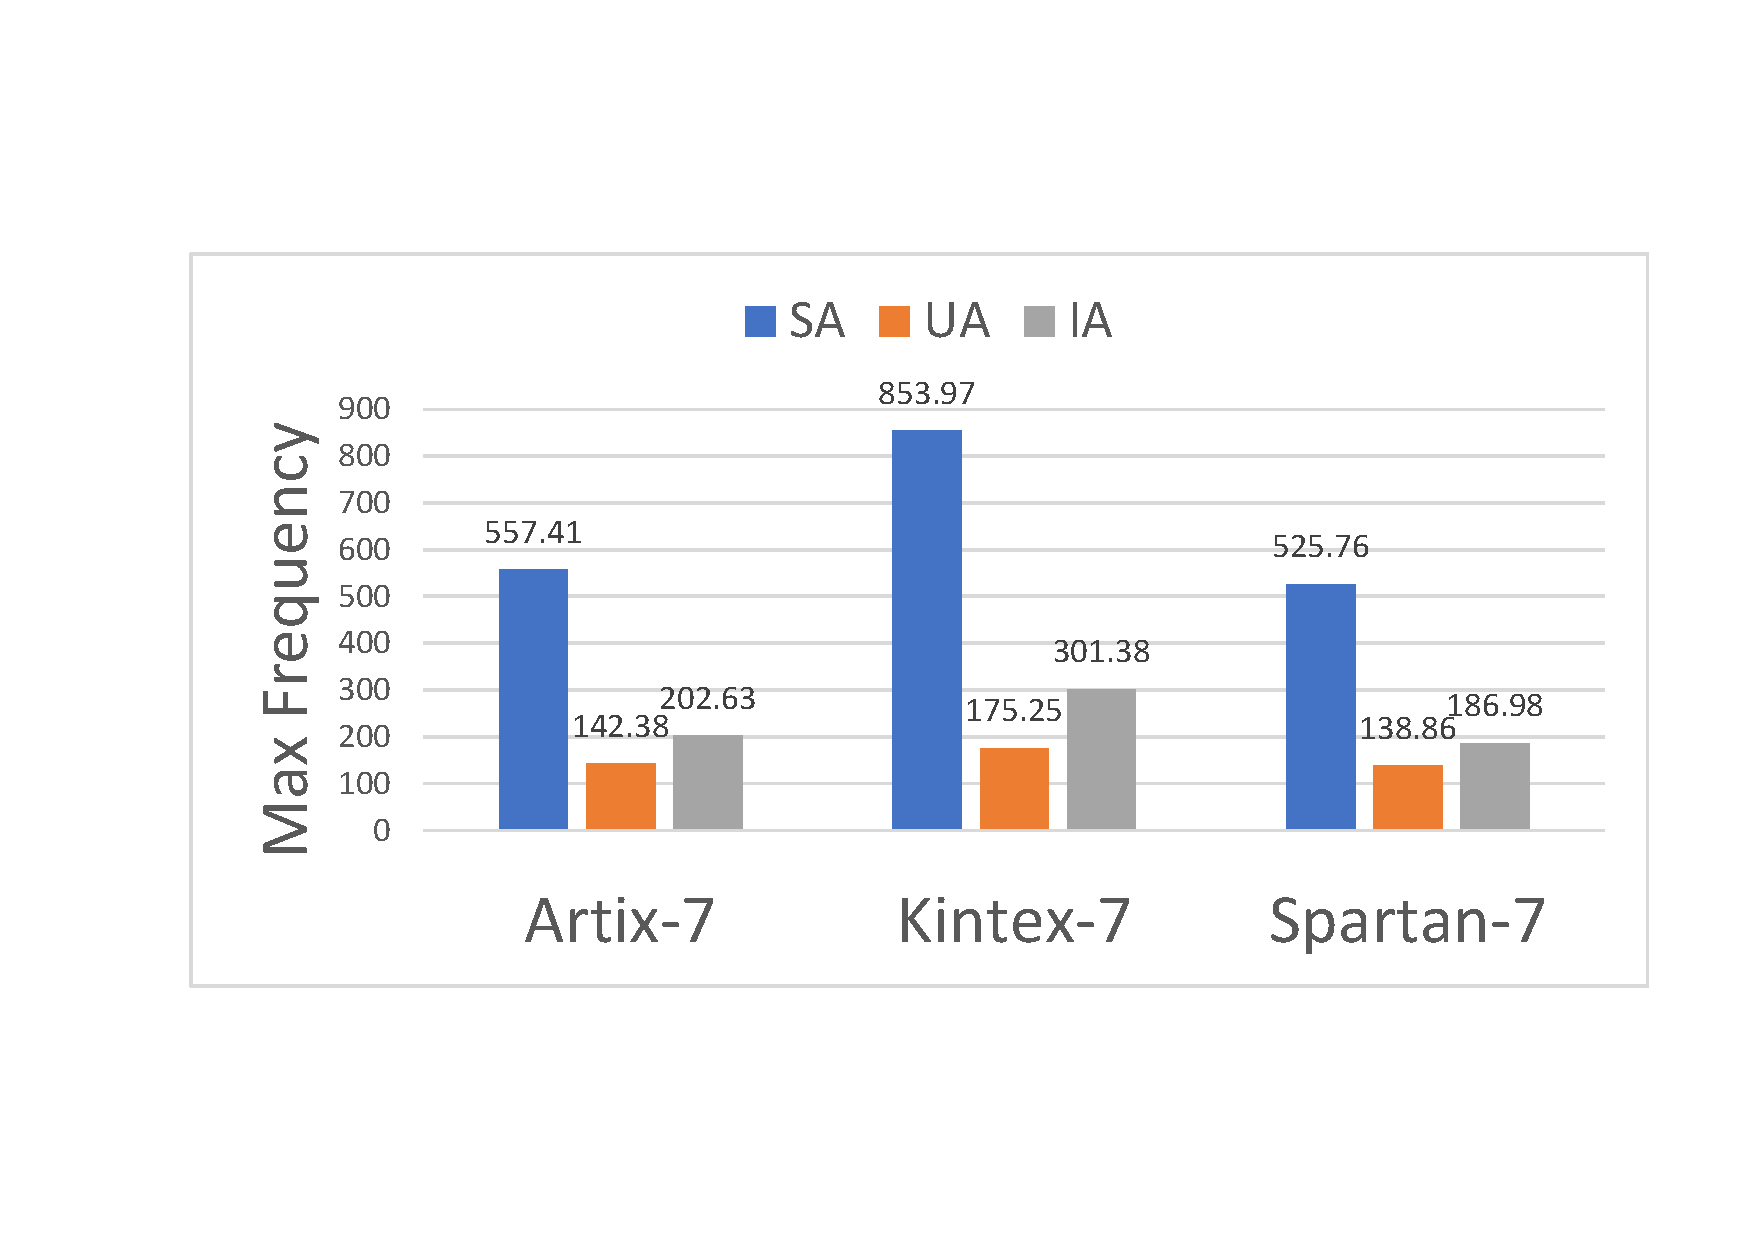
\includegraphics[width=0.45\textwidth]{./fig/compare-maxf.pdf}
    \caption{Comparison of Max Frequency in Three Architectures}\label{compare-maxF}
\end{figure}

The serial architecture has the highest energy per bit due to its higher latency, which results in the smallest area. Conversely, the unrolled architecture has the lowest energy per bit because it has the lowest latency. The energy per bit of the iterative architecture of PRESENT falls between that of the serial architecture and the unrolled architecture. Compared to the iterative architecture of PRESENT, the unrolled architecture reduces energy per bit by 47.89\%. Figure~\ref{compare-energy} illustrates the energy per bit for the three architectures.

\begin{figure}
    \centering
    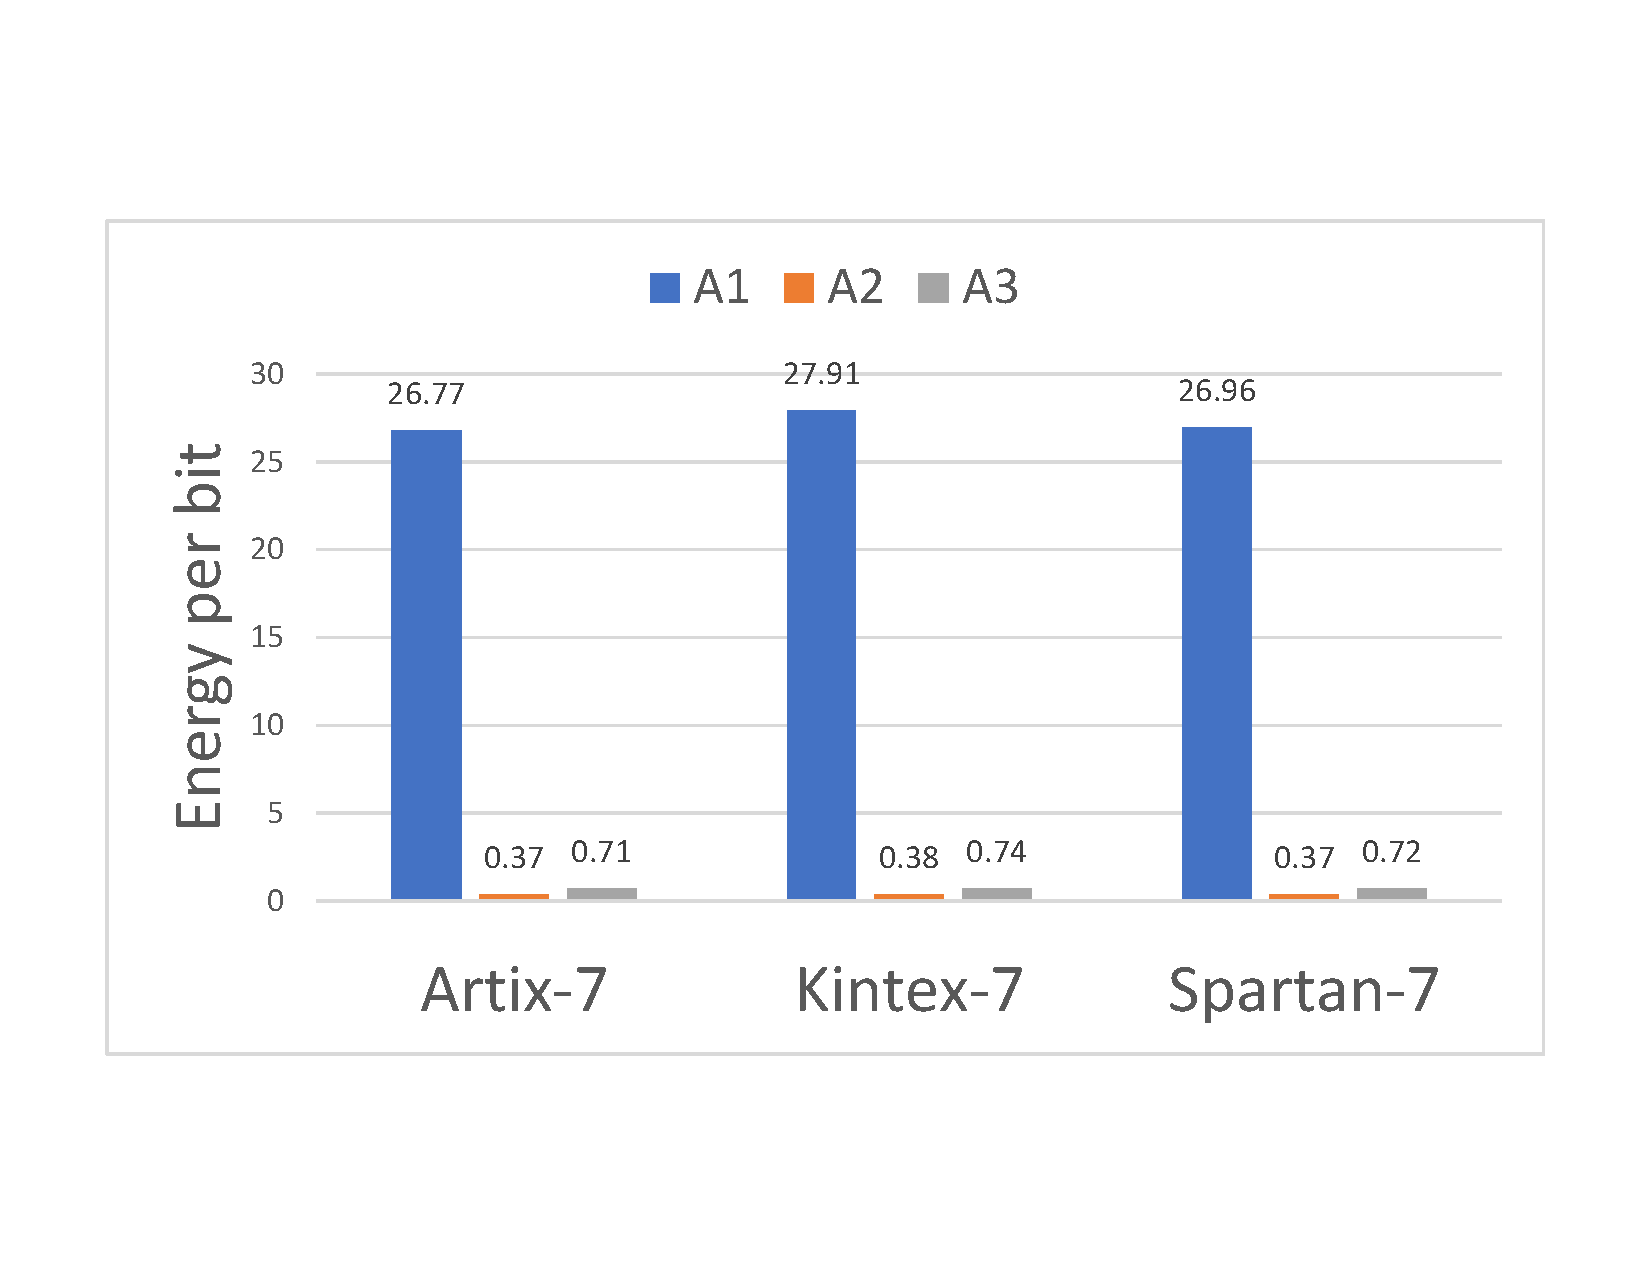
\includegraphics[width=0.45\textwidth]{./fig/compare-energy.pdf}
    \caption{Comparison of Energy Per Bit in Three Architectures}\label{compare-energy}
\end{figure}


\section{Conclusion}\label{sec6}

Given the diverse performance requirements arising from the use of IoT devices in various contexts, achieving optimal security without compromising performance presents a significant challenge. Implementing effective solutions is one way to attain this balance between security and performance.

This research presents two unique designs for the CRAFT Lightweight cipher - Serial and Unrolled - both aimed at boosting performance.
The Serial architecture reduces the area consumption by 15.72\% compared to the iterative architecture of PRESENT.
The Unrolled architecture, on the other hand, reduces the latency to 16, effectively doubling the throughput rate at 100MHz compared to the iterative architecture of PRESENT.
Additionally, the Unrolled architecture reduces energy per bit by 47.89\% compared to the iterative architecture of PRESENT.
To the best of our knowledge, the Serial architecture establishes a new record for area efficiency on an FPGA configured with a 64-bit block size and 128-bit key size. 
These proposed architectures are therefore highly suitable for environments with IoT devices.

Future work could involve investigating the application of these proposed architectures in real-world IoT devices and measuring their performance. Additionally, implementing these architectures on ASICs could further reduce area consumption.

\bibliographystyle{elsarticle-num}
\bibliography{bibliography}

\end{document}
\endinput
%%
%% End of file `elsarticle-template-num.tex'.
